% Arquivo LaTeX de exemplo de dissertação/tese a ser apresentada à CPG do IME-USP
%
% Criação: Jesús P. Mena-Chalco
% Revisão: Fabio Kon e Paulo Feofiloff
% Adaptação para UTF8, biblatex e outras melhorias: Nelson Lago
%
% Except where otherwise indicated, these files are distributed under
% the MIT Licence. The example text, which includes the tutorial and
% examples as well as the explanatory comments in the source, are
% available under the Creative Commons Attribution International
% Licence, v4.0 (CC-BY 4.0) - https://creativecommons.org/licenses/by/4.0/


%%%%%%%%%%%%%%%%%%%%%%%%%%%%%%%%%%%%%%%%%%%%%%%%%%%%%%%%%%%%%%%%%%%%%%%%%%%%%%%%
%%%%%%%%%%%%%%%%%%%%%%%%%%%%%%% PREÂMBULO LaTeX %%%%%%%%%%%%%%%%%%%%%%%%%%%%%%%%
%%%%%%%%%%%%%%%%%%%%%%%%%%%%%%%%%%%%%%%%%%%%%%%%%%%%%%%%%%%%%%%%%%%%%%%%%%%%%%%%

% A opção twoside (frente-e-verso) significa que a aparência das páginas pares
% e ímpares pode ser diferente. Por exemplo, as margens podem ser diferentes ou
% os números de página podem aparecer à direita ou à esquerda alternadamente.
% Mas nada impede que você crie um documento "só frente" e, ao imprimir, faça
% a impressão frente-e-verso.
%
% Aqui também definimos a língua padrão do documento (a última da lista) e
% línguas adicionais. Para teses do IME, no mínimo português e inglês são
% obrigatórios, porque independentemente da língua principal do texto é
% preciso fornecer o resumo nessas duas línguas. LaTeX aceita alguns nomes
% diferentes para a língua portuguesa; dentre as opções, prefira sempre
% "brazilian" para português brasileiro e "portuguese" para português europeu.
\documentclass[a4paper,12pt,twoside,brazilian,english]{book}
% \documentclass[a4paper,12pt,twoside,english,brazilian]{book}

% O preâmbulo de um documento LaTeX pode ser razoavelmente longo. Neste
% modelo, optamos por reduzi-lo, colocando praticamente tudo do preâmbulo
% nas packages "imegoodies" e "imelooks".
%
% imegoodies carrega diversas packages muito úteis e populares (algumas
% são praticamente obrigatórias, como amsmath, babel, array etc.). É
% uma boa ideia usá-la com outros documentos também. Ela inclui vários
% comentários explicativos e dicas de uso; não tenha medo de alterá-la
% conforme a necessidade.
%
% imelooks carrega algumas packages e configurações que definem a
% aparência do documento; você também pode querer usá-la (ou partes
% dela) com outros documentos para obter as mesmas fontes, margens
% etc. Tal como "imegoodies", pode valer a pena ler os comentários
% e fazer modificações nessa package. Com a opção "thesis", imelooks
% também define os comandos para capa, folha de rosto etc.
\usepackage{imegoodies}
\usepackage[thesis]{imelooks}

%\nocolorlinks % para impressão em P&B

% Diretórios onde estão as figuras; com isso, não é necessário (mas
% é permitido) colocar o caminho completo em \includegraphics. Note
% que a extensão nunca é necessária (mas é permitida), ou seja, o
% resultado é o mesmo com "\includegraphics{figuras/foto.jpeg}",
% "\includegraphics{foto.jpeg}", "\includegraphics{figuras/foto}"
% ou "\includegraphics{foto}".
\graphicspath{{figuras/},{fig/},{logos/},{img/},{images/},{imagens/}}

% Comandos rápidos para mudar de língua:
% \en -> muda para o inglês
% \br -> muda para o português
% \texten{blah} -> o texto "blah" é em inglês
% \textbr{blah} -> o texto "blah" é em português
\babeltags{en = english, br = brazilian}


%%%%%%%%%%%%%%%%%%%%%%%%%%%%%%%%%%%%%%%%%%%%%%%%%%%%%%%%%%%%%%%%%%%%%%%%%%%%%%%%
%%%%%%%%%%%%%%%%%%%%%%%%%%%%%%%%%% METADADOS %%%%%%%%%%%%%%%%%%%%%%%%%%%%%%%%%%%
%%%%%%%%%%%%%%%%%%%%%%%%%%%%%%%%%%%%%%%%%%%%%%%%%%%%%%%%%%%%%%%%%%%%%%%%%%%%%%%%

% O arquivo com os dados bibliográficos para biblatex; você pode usar
% este comando mais de uma vez para acrescentar múltiplos arquivos
\addbibresource{bibliografia.bib}

% Este comando permite acrescentar itens à lista de referências sem incluir
% uma referência de fato no texto (pode ser usado em qualquer lugar do texto)
%\nocite{bronevetsky02,schmidt03:MSc, FSF:GNU-GPL, CORBA:spec, MenaChalco08}
% Com este comando, todos os itens do arquivo .bib são incluídos na lista
% de referências
%\nocite{*}

% É possível definir como determinadas palavras podem (ou não) ser
% hifenizadas; no entanto, a hifenização automática geralmente funciona bem
\babelhyphenation{documentclass latexmk soft-ware clsguide} % todas as línguas
\babelhyphenation[brazilian]{Fu-la-no}
\babelhyphenation[english]{what-ever}

% Estes comandos definem o título e autoria do trabalho e devem sempre ser
% definidos, pois além de serem utilizados para criar a capa, também são
% armazenados nos metadados do PDF. O subtítulo é opcional.
\title{Case Studies in Microservices towards Extensibility}

\author{Gabriel Fernandes Mota}

% Para TCCs, este comando define o supervisor
\orientador{Prof. Dr. Eduardo Guerra}

% Se não houver, remova; se houver mais de um, basta
% repetir o comando quantas vezes forem necessárias
\coorientador{MSc. João Francisco Lino Daniel}

% A página de rosto da versão para depósito (ou seja, a versão final
% antes da defesa) deve ser diferente da página de rosto da versão
% definitiva (ou seja, a versão final após a incorporação das sugestões
% da banca).
\tipotese{
  % mestrado,
  %doutorado,
  tcc,
  %definitiva, % É a versão para defesa ou a versão definitiva?
  %quali, % É qualificação?
  programa={Ciência da Computação},
}

\defesa{
  local={São Paulo},
  data=2024-12-03, % YYYY-MM-DD
}

% A licença do seu trabalho. Use CC-BY, CC-BY-NC, CC-BY-ND, CC-BY-SA,
% CC-BY-NC-SA ou CC-BY-NC-ND para escolher a licença Creative Commons
% correspondente (o sistema insere automaticamente o texto da licença).
% Se quiser estabelecer regras diferentes para o uso de seu trabalho,
% converse com seu orientador e coloque o texto da licença aqui, mas
% observe que apenas TCCs sob alguma licença Creative Commons serão
% acrescentados ao BDTA. Se você tem alguma intenção de publicar o
% trabalho comercialmente no futuro, sugerimos a licença CC-BY-NC-ND.
%
%\direitos{CC-BY-NC-ND}
%
%\direitos{Autorizo a reprodução e divulgação total ou parcial deste
%          trabalho, por qualquer meio convencional ou eletrônico,
%          para fins de estudo e pesquisa, desde que citada a fonte.}
%
%\direitos{I authorize the complete or partial reproduction and disclosure
%          of this work by any conventional or electronic means for study
%          and research purposes, provided that the source is acknowledged.}
%
\direitos{CC-BY}


%%%%%%%%%%%%%%%%%%%%%%%%%%%%%%%%%%%%%%%%%%%%%%%%%%%%%%%%%%%%%%%%%%%%%%%%%%%%%%%%
%%%%%%%%%%%%%%%%%%%%%%% AQUI COMEÇA O CONTEÚDO DE FATO %%%%%%%%%%%%%%%%%%%%%%%%%
%%%%%%%%%%%%%%%%%%%%%%%%%%%%%%%%%%%%%%%%%%%%%%%%%%%%%%%%%%%%%%%%%%%%%%%%%%%%%%%%

\begin{document}

%%%%%%%%%%%%%%%%%%%%%%%%%%% CAPA E PÁGINAS INICIAIS %%%%%%%%%%%%%%%%%%%%%%%%%%%%

% Aqui começa o conteúdo inicial que aparece antes do capítulo 1, ou seja,
% página de rosto, resumo, sumário etc. O comando frontmatter faz números
% de página aparecem em algarismos romanos ao invés de arábicos e
% desabilita a contagem de capítulos.
\frontmatter

\pagestyle{plain}

\onehalfspacing % Espaçamento 1,5 na capa e páginas iniciais

\maketitle % capa e folha de rosto

%%%%%%%%%%%%%%%% DEDICATÓRIA, AGRADECIMENTOS, RESUMO/ABSTRACT %%%%%%%%%%%%%%%%%%

% Reinicia o contador de páginas (a próxima página recebe o número "i") para
% que a página da dedicatória não seja contada.
\pagenumbering{roman}

%!TeX root=../tese.tex
%("dica" para o editor de texto: este arquivo é parte de um documento maior)
% para saber mais: https://tex.stackexchange.com/q/78101

% As palavras-chave são obrigatórias, em português e em inglês, e devem ser
% definidas antes do resumo/abstract. Acrescente quantas forem necessárias.

\keywords{Microservices,Extensibility,Non-functional requirements,Software Architecture}

\palavraschave{Microserviços, Extensibilidade, Requisitos não-funcionais, Arquitetura de Software}

\abstract{
 Microservices is an architecture pattern that has increased in popularity since the 2010s for its benefits in scalability and context boundaries for big systems. Nowadays, tech companies use continuous delivery to create ever-growing systems that keep evolving. Microservices are usually used in these systems, for the ability to add new services to extend systems functionalities. However, there is a lack of formal knowledge about it towards non-functional requirements besides scalability. 
 This work explores the concept of extensibility, a non-functional requirement for systems that need to have their function extended in a new feature, keeping the same responsibility.
 To do so, we study two microservices’ case studies, a Data Provider and a Data Ingestion system—each one with different architecture approaches implemented. The implementation provided runtime metrics and developer experience to compare them, mainly regarding extensibility. 
In the end, the results of the case studies pointed to the benefits of three highlights: (i) the asynchronous approach for internal communication, (ii) the usage of metadata for the integration of heterogeneous systems, and (iii) the data replication to reduce external chattiness.    
}

% O resumo é obrigatório, em português e inglês. Estes comandos também
% geram automaticamente a referência para o próprio documento, conforme
% as normas sugeridas da USP.
\resumo{
 Microserviços é um padrão arquitetural que tem aumentado em popularidade no últimos anos devido a seus benefícios em relação à escalabilidade e limite de contexto para grandes sistemas. Atualmente, empresas de tecnologia usam entrega contínua para criar sistemas que continuam crescendo e evoluindo. Microserviços são comumente usados junto, pela capacidade de adicionar novos serviços e estender as funcionalidades do sistema. Porém, há uma falta de conhecimento formal sobre o assunto em relação a requisitos não-funcionais além de escalabilidade.
 Esse trabalho explora o conceito de extensiblidade, um requisito não-funcional para sistemas que precisam estender suas funcionalidades, mantendo as mesmas responsabilidades.
 Para fazer isso, estudamos dois casos de microserviços, um Provedor de Dados e um sistema de Ingestão de Dados—cada um com diferentes arquiteturas implementadas. Cada implementação forneceu métricas durante a execução do sistema e de expêriencia de desenvolvimento para comparar as arquiteturas, principalmente em quesito a extensibilidade.
 No final, os resultados dos caso de estudos apontaram para benefícios em três conceitos: (i) uso de comunicação assíncrona interna entre os serviços, (ii) uso de metadados para integração de sistemas heterogêneos, e (iii) a replicação de dados para reduzir comunição desnecessária entre os serviços.
}


%%%%%%%%%%%%%%%%%%%%%%%%%%% LISTAS DE FIGURAS ETC. %%%%%%%%%%%%%%%%%%%%%%%%%%%%%

% Como as listas que se seguem podem não incluir uma quebra de página
% obrigatória, inserimos uma quebra manualmente aqui.
\cleardoublepage

% Todas as listas são opcionais; Usando "\chapter*" elas não são incluídas
% no sumário. As listas geradas automaticamente também não são incluídas por
% conta das opções "notlot" e "notlof" que usamos para a package tocbibind.

% Normalmente, "\chapter*" faz o novo capítulo iniciar em uma nova página, e as
% listas geradas automaticamente também por padrão ficam em páginas separadas.
% Como cada uma destas listas é muito curta, não faz muito sentido fazer isso
% aqui, então usamos este comando para desabilitar essas quebras de página.
% Se você preferir, comente as linhas com esse comando e des-comente as linhas
% sem ele para criar as listas em páginas separadas. Observe que você também
% pode inserir quebras de página manualmente (com \clearpage, veja o exemplo
% mais abaixo).
\newcommand\disablenewpage[1]{{\let\clearpage\par\let\cleardoublepage\par #1}}

% Nestas listas, é melhor usar "raggedbottom" (veja basics.tex). Colocamos
% a opção correspondente e as listas dentro de um grupo para ativar
% raggedbottom apenas temporariamente.
\bgroup
\raggedbottom

%%%%% Listas criadas automaticamente

% Sumário (obrigatório)
\tableofcontents

\egroup % Final de "raggedbottom"

%%%%%%%%%%%%%%%%%%%%%%%%%%%%%%%% CAPÍTULOS %%%%%%%%%%%%%%%%%%%%%%%%%%%%%%%%%%%%%

% Aqui vai o conteúdo principal do trabalho, ou seja, os capítulos que compõem
% a dissertação/tese. O comando mainmatter reinicia a contagem de páginas,
% modifica a numeração para números arábicos e ativa a contagem de capítulos.
\mainmatter

\pagestyle{mainmatter}

% Espaçamento simples
\singlespacing

\pagestyle{mainmatter}
\chapter{Introduction}
\label{cap:introduction}

\enlargethispage{.5\baselineskip}

The concept of building applications with loosely coupled services emerged in 1997 on IBM's Enterprise Java Bean (EJB). However, it was only with the REST APIs growth in the early 2010s that microservices were popularized as an established architecture for large systems requiring fast growth, continuous integration, and scalability.

As a recent software architecture style, it lacks formal knowledge and experimentation in some areas, such as its patterns and API interfaces, inter-service communication, and data management.

Extensibility is the capability of a component to extend its functionality to similar uses. An extensible system can help developers reduce work to implement new features, and architects reuse components to create simpler solutions.

Microservices can help with extensibility because of modularization and single-responsibility attached to each microservice. Allowing systems to apply extensibility only on key services for, and impact the whole architecture.

This work studies multiple microservices use cases, from a developer and architect perspective, exploring the concept of extensibility and other non-functional requirements, regarding services’ contracts, communication, and management.
%!TeX root=../tese.tex
%("dica" para o editor de texto: este arquivo é parte de um documento maior)
% para saber mais: https://tex.stackexchange.com/q/78101

%% ------------------------------------------------------------------------- %%

\chapter{Literature Review}
\label{cap:literature}

\enlargethispage{.5\baselineskip}

\section{Metrics}
\label{sec:metrics}
Metrics are a representation of an object’s characteristic as a numeric value~\cite{OOMetrics}. In association with units of measurement and thresholds, metrics are used to describe the object and also to assess it.

In software development, metrics are used to describe many aspects of a system, from objective characteristics – like response time and CPU usage, that have standards and well-defined ways of measurement –, to subjective ones – like code quality and software maintainability, which can be measured by several methods, each one of them with its own efficiency and accuracy.

The assessment made with metrics can go in different directions, such as to track if a certain goal has been achieved, or to follow if a specific requirement is being respected. In general, different metrics can be used to assess a single characteristic, but the choice depends on the goal of the analysis. For example, to represent the degree of coupling between modules A and B, we can use the static number of function calls, or we can use the dynamic number of calls per minute during execution.

\section{Software Architecture}
\label{sec:softarq}
Software Architecture is an area of study in computer science that focus on the software structures, their benefits and drawbacks, and how to integrate them to solve problems~\cite{SoftArch}.

The architecture of a software is what describes which set of structures are used to build a system, encompassing its components, principles, responsibilities and design decisions. It doesn't necessarily establish implementation details, like technologies, design patterns and intra-component architecture, it depends on the level of detail and how big is the whole structure. However, all decisions taken in the architecture should be all necessary to reason about the software and its implementation.

\subsection*{Non-functional Requirements}
\label{sec:nonfunctional}
When defining a software's architecture, there are a set of requirements that should be fulfilled, so the software solves the problem it was intended to. These requirements can be split in two groups: functional and non-functional. Functional requirements describe what the software should do, the behavior. Non-functional requirements define how this should be done, the qualities.

Non-functional requirements should be as well-defined as the functional ones. For example, a live chat API should allow two users to interact with each other at the same time, with a maximum 500ms delay to message deliver. This not only defines what is the API functionality, but also that it should be performant, and this requirement is as important as the functionality, since an API with slow response time does not fully solve the problem.

\subsection*{Extensibility}
\label{sec:extensibility}
Quality of what can be extended~\cite{Evoluctionary}. In the context of software, a system or architecture can be said extensible if it is able to receive new features without requiring major changes. 

Features are capacities added to a component that doesn't change its functionality. Extensibility should be achieved without violating the single-responsability principle.

For example, a component designed to translate text from portuguese to english, can be said extensibile if it doesn't require major changes to implement translation from portuguese to spanish. The system does a new thing, however it still with the single functionality of translating.

\section{Microservices}
\label{sec:microservices}
In the past, the development of a software system could be explained as a line, with planning, beginning and an ending delivery. With technology advances, continuous delivery emerged, turning this process into a cycle that can be repeated without never reaching a final delivery. In this scenario, companies started to have problem scaling large monolithic applications, because they require knowledge about all the system for changes, this knowledge usually ended up concentrated in a few developers that took part on the building of the application. This leads to business changes being held by engineering limitation. Microservice comes up as a solution that allow fast pace development in large systems and fits better the necessities of a fast delivery market. 

Microservice is a software architecture style, in which, the responsibilities and business functionalities are split into independently deployable components, each component has its own codebase and is called a "microservice"~\cite{Micro}. These services communicate through APIs, Application Programming Interfaces, these interfaces work as contracts, containing rules, protocols and tools, that other services may follow to be able to communicate with it.

Microservices components follow the rule of single responsibility, each component is responsible for doing only one thing and must do it well. This allows organizations to split the concerns in multiple cores, each with its own sets of services where the ramp up and specialization is easier, since it can be focused on specific area. For example, a common split of teams on big techs is in functional areas: mobile client, web client, data management, back-end development, etc.

It also allows splitting the decision in multiple layers. While a software architect may be responsible for defining which services take part of a certain flow, and what are their responsibilities, the technical and design decisions of implementation can be made by the maintainer development team, since each component is technology independent.

Another advantage of microservice is scalability and extensibility. As components are independent, you can cut cost by scaling only the required components at a time. It also means that, adding a new feature can be as easy as creating a new independent service and attaching it to the architecture.

However, this architecture relies on inter-components contracts, which means that any break in a contract can lead to a cascade of unwanted behaviors that require lots of tracking and measurements to debug. It also requires an increase in design complexity and operational cost due to the necessity of handling multiple services, their deployment and integration.

\chapter{Methodology}

The goal of this work is to explore the concept of extensibility on MSA, and Microservice Architecture, and understand which components and concepts are key to developing an extensible software system. To reach it, we study two software use cases with different MSA solutions, comparing each solution regarding design, development, and execution.

To do so, the study was done in an iterative process with solution design, architecture implementation, metrics collection, and evaluation, inspired by Design Science Research(~\cite{DesignParad}).

\begin{figure}
    \centering
    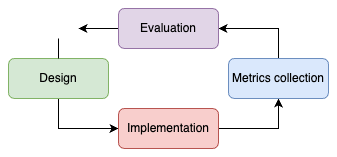
\includegraphics[width=.8\textwidth]{collector-consumer-Methodology.drawio}
    \caption{Methodology cycle.\label{fig:subfigures1}}
\end{figure}

During the solution design, we set the use case that is going to be studied and which architecture solutions, or scenarios, we want to explore. Then, the architecture's microservices are implemented and integrated locally. Once the application is ready, it is executed on different tests according to the study case and metrics are collected in regards to development experience and runtime measurements. At the end of the iteration, the scenarios are compared and the metrics collected are evaluated.

\begin{figure}
    \centering
    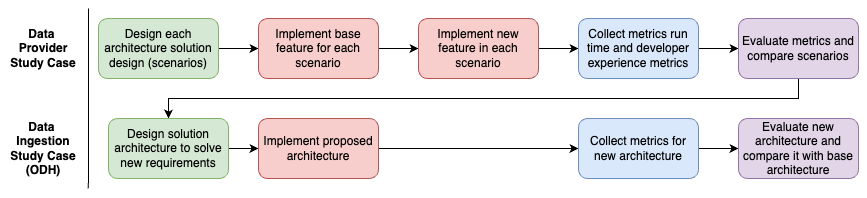
\includegraphics[width=1\textwidth]{collector-consumer-Methodology cycle.drawio}
    \caption{Iterations.\label{fig:subfigures2}}
\end{figure}

It was done in two iterations, each iteration was a case study where the use of microservices is required and extensibility is a non-functional requirement.

The first iteration was based on a common feature from multiple systems: a service dedicated to handling access and serving data from common data storage to different clients. We named this case as “Data Provider”.

An initial solution is to protect the data source by exposing it as a service. The clients then access it via a REST API using a polling strategy. This study case compares it with two asynchronous approaches: a registration system that implements internally the broadcasting of the data exposed as REST API, and an event-based communication that delegates the broadcasting to a message broker.

The iteration started with the implementation of each scenario on a SpringBoot application according to the following GitHub pull requests:

\begin{itemize}
    \item Polling gateway implementation: https://github.com/gfmota/charging-plug-gateway/pull/4
    \item Broadcaster gateway implementation: https://github.com/gfmota/charging-plug-gateway/pull/6
    \item Message-broker based implementation: https://github.com/gfmota/charging-plug-gateway/pull/1
\end{itemize}

Then, we wanted to compare the technical effort necessary to extend the features in each scenario. So, we extended each scenario with a new microservice.

\begin{itemize}
    \item Polling provider new feature implementation: https://github.com/gfmota/charging-plug-gateway/pull/5
    \item Broadcaster provider new feature implementation: https://github.com/gfmota/charging-plug-gateway/pull/7
    \item Message-broker provider new feature implementation: https://github.com/gfmota/charging-plug-gateway/pull/8
\end{itemize}

During development, we collected developer experience metrics from a junior software engineer developing each provider. Such as, the number of lines changed and knowledge necessary for each scenario. Due to the small sample, this may contain bias, and we encourage the experiment with a larger sample and a bigger context. 

After the implementation, each scenario was run locally in three clients' usage battery, with 10, 100, and 1000 clients simultaneously for each one of the three data types provided. During runtime, we collected the application’s health metrics from the data provider, such as CPU and memory usage, success, and database access rate.

Then, we used the developer experience and runtime metrics to compare each scenario in regard to extensibility, scalability, data source usage, client autonomy, and infrastructure cost.  

On the second iteration, the work studied OpenDataHub's Data Ingestion use case. The Data Ingestion system is composed of several applications dedicated to collecting and receiving data from multiple external sources, transforming them into a standardized structure, and saving on common data storage.

We talked with OpenDataHub's team to understand the current architecture, the requirements it met, and the desired requirements that are currently unfulfilled. 

Then, we designed a new architecture to accommodate both the old and the new requirements and implemented it as follows on GitHub's repository https://github.com/gfmota/data-ingestion-monorepo.

The implementation contains the integration of an Austrian Geosphere dataset, provided by the OpenDataHub's team, as an example.

The implementation is used to simulate dataset integration, active and passive integration, and to collect some analytical data about the new architecture. Then, we compared the current and the proposed architecture theoretically in regard to extensibility, the work necessary to integrate a new dataset, and the system's functional requirements.

\newcommand{\sla}{\textbackslash}

\newcommand{\cmd}[1]{\textsf{#1}}

\newcommand{\pkg}[1]{\textsf{#1}}

\newcommand{\ltxcmd}[1]{\cmd{\sla{}#1}}

\chapter{Data Provider Study Case}
\label{chap:dataprovider}

\section{Introduction}
\label{sec:introductionprov}

This study case explores a Data Provider requirement. A Data Provider is a service dedicated to handle access and serve data from a data storage to multiple clients. Each client may have different needs on which set of data or data update frequency, the Data Provider must be able to handle it and to provide the data requested.

This exploration is made by an experiment in which three different architectures, scenarios, that solve the Data Provider requirement – contain a service that fetches data and serves it to multiple independent clients. At the end, there is a comparison between each one in regard to how well they fit new features in the format of clients consuming new data type. Exploring points such as performance, developer experience, client autonomy and infrastructure.

In this experiment, each scenario have the same requirements of implementing the same three components, they differ on the communication between components. The three components that compose the experiment:

{Data Consumers}
\label{sec:dataconsumer}

Also mentioned as \textbf{client} or \textbf{data analyzer}

This is a group of services that need the data. They are independent of each other and may have different needs of data. What they do with the data does not matter for the experiment, for this reason, they are only going to log the values received and are simple services implemented in Java with SpringBoot. https://github.com/gfmota/charging-plug-data-analyzer

\subsection*{Data Provider}
\label{sec:dataprovider}

Also mentioned as \textbf{gateway}

It is responsible for querying the data on the data source, formatting, handling any business logic associated to it, and serving it to the client. They are implemented in Java as a SpringBoot application, but it could be used any technology with capacity to make and receive HTTP requests, and connect to a message queue-based asynchronous communication tool. https://github.com/gfmota/charging-plug-gateway

\subsection*{Data lake}
\label{sec:datalake}

Also mentioned as \textbf{data source}

The chosen was a third party API, Open Data Hub Mobility API https://docs.opendatahub.com/en/latest/index.html, that makes available data about charging plug station for automobiles from Europe.\footnote{Endpoint used to request data for the Data Lake: https://swagger.opendatahub.com/?url=https://mobility.api.opendatahub.com/v2/apispec#/Mobility using different queries according to client needs.}

However, the data source type doesn't matter, it could be a search engine or conventional database that it wouldn't affect what this experiment aims to measure. It was chosen for reasons of ease to plug-in and use, and the amount of data available.   

\section{Scenarios}
\label{sec:scenarios}

Each scenario corresponds to an architectural design that solves the problem of a data source gateway. For each scenario, there are two development cycles, the gateway development with two base features, and the next one adds a new feature as a third data type, used to final comparisons.

\subsection*{Polling-based gateway}
\label{sec:polling}

In this scenario, the gateway works as a synchronous read-only API in which the clients can query the data with HTTP requests. The gateway acts as an Adapter for the data source, where each type of data has its own endpoint. The clients are responsible for requesting the data it wants; the gateway translates the received request into a query to the data source, and formats its response before sending back to the client. The base implementation is detailed at the pull request: https://github.com/gfmota/charging-plug-gateway/pull/4

\begin{figure}
    \centering
    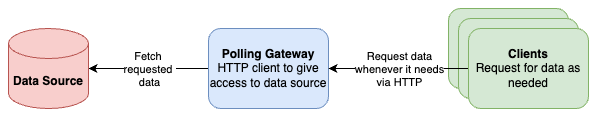
\includegraphics[width=1\textwidth]{Gateway-Pooling Gateway.drawio}
    \caption{Pooling Gateway Architecture.\label{fig:subfigures3}}
\end{figure}

\subsection*{Broadcaster gateway}
\label{sec:broadcaster}

In this scenario, the gateway provides a subscription service with asynchronous message sender API. Each consumer can subscribe to the gateway by registering its desired data and address, and the gateway notifies on triggers. These messages and subscription are made with HTTP requests. Note that the data provider needs some type of storage to keep track of the subscribed services. For this implementation, it uses a CSV file, but it could be any other most usual database. The base implementation is detailed at the pull request: https://github.com/gfmota/charging-plug-gateway/pull/6

\begin{figure}
    \centering
    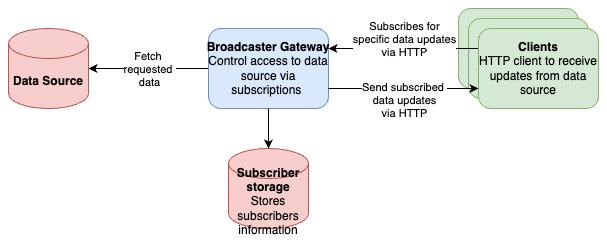
\includegraphics[width=1\textwidth]{Gateway-Broadcaster Gateway.drawio}
    \caption{Broadcaster Gateway Architecture.\label{fig:subfigures4}}
\end{figure}

{Message queue-based gateway}
\label{sec:messagequeue}

In this scenario, the data provider offers an asynchronous event-notifier API to provide data to the consumers. The data provider retrieves the data upon triggers and post it to a topic as a message with a tag that specifies the type of data it contains. Each data consumer is responsible for creating its own queue and attaching it to the topic with the correct message tag according to the data it wants. This implementation uses RabbitMQ, but it could be any other broker with topic implementation. The base implementation is detailed at the pull request: https://github.com/gfmota/charging-plug-gateway/pull/2

\begin{figure}
    \centering
    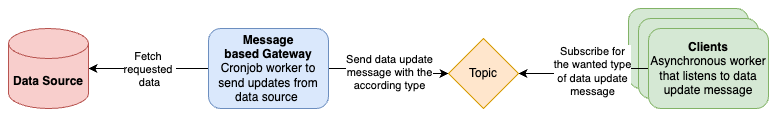
\includegraphics[width=1\textwidth]{Gateway-Message based Gateway.drawio}
    \caption{Message queue-based Gateway Architecture.\label{fig:subfigures5}}
\end{figure}

\section{Execution}
\label{sec:execution}

To run the experiment, it was created a repository with gateway and analyzer repositories, and scripts to run each scenario. https://github.com/gfmota/charging-plug-experiment

\begin{program}
    \index{Bash}
    \centering
  
  \begin{lstlisting}[language=bash, style=wider]
    ./run_polling_experiment.sh
  \end{lstlisting}
  
    \caption{Command to run polling scenario.\label{prog:java1}}
\end{program}

\begin{program}
    \index{Bash}
    \centering
  
  \begin{lstlisting}[language=bash, style=wider]
    ./run_broadcaster_experiment.sh
  \end{lstlisting}
  
    \caption{Command to run broadcaster scenario.\label{prog:java2}}
\end{program}

\begin{program}
    \index{Bash}
    \centering
  
  \begin{lstlisting}[language=bash, style=wider]
    ./run_message_experiment.sh
  \end{lstlisting}
  
    \caption{Command to run message based scenario.\label{prog:java3}}
\end{program}

All of them can receive an integer parameter to define the amount of clients the gateway will handle simultaneously, this doesn't mean that it will run n clients application, but a single application that will mimic n clients.

These scripts run the gateway and client application on ports 8080 and 8081 respectively, and also makes available metrics graphs on Grafana that you can access at port 3000 at /dashboard (login is admin/admin). These metrics are going to be used to evaluate how the gateway's performance behavior with multiple clients and different features.

There is also applications' log on /log to debug any unexpected behavior.

On polling experiment, instead of using the analyzer, it was replaced by jmeter, a load testing tool, highly configurable, that can simulate multiple HTTP clients requesting data at the same time.

\section{Results}
\label{sec:results}

The results contain the amount of changes necessary during the second development cycle and the Grafana's dashboards after multiple execution with different amount of clients to serve, 10, 100 and 1000..

Every board contains graphs of CPU and memory percentage usage by the application, and a graph with the amount of data access according to the Open Data Hub time of information: last status is used by current status feature, and time range is used by daily and hourly report.

\subsection*{Polling gateway}
\label{sec:pollingresult}

The code necessary to implement the new feature at the Polling gateway is at this PR https://github.com/gfmota/charging-plug-gateway/pull/5 (Figure~\ref{fig:pollingdif})

\begin{figure}
    \centering
    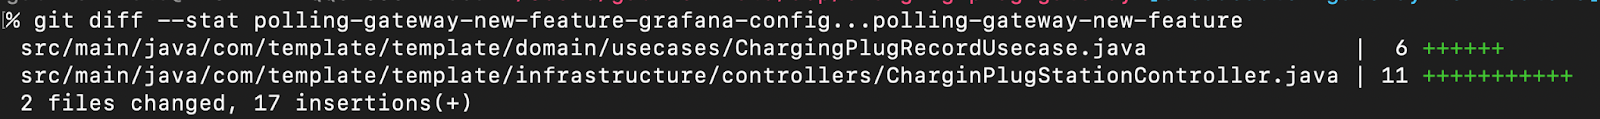
\includegraphics[width=1\textwidth]{pollingdif}
    \caption{Polling gateway extension code diff.\label{fig:pollingdif}}
\end{figure}

The execution of the experiment consists of a jmeter load test with 10, 100 and 1000 clients to simulate different clients at the same time.

\begin{figure}
    \centering
    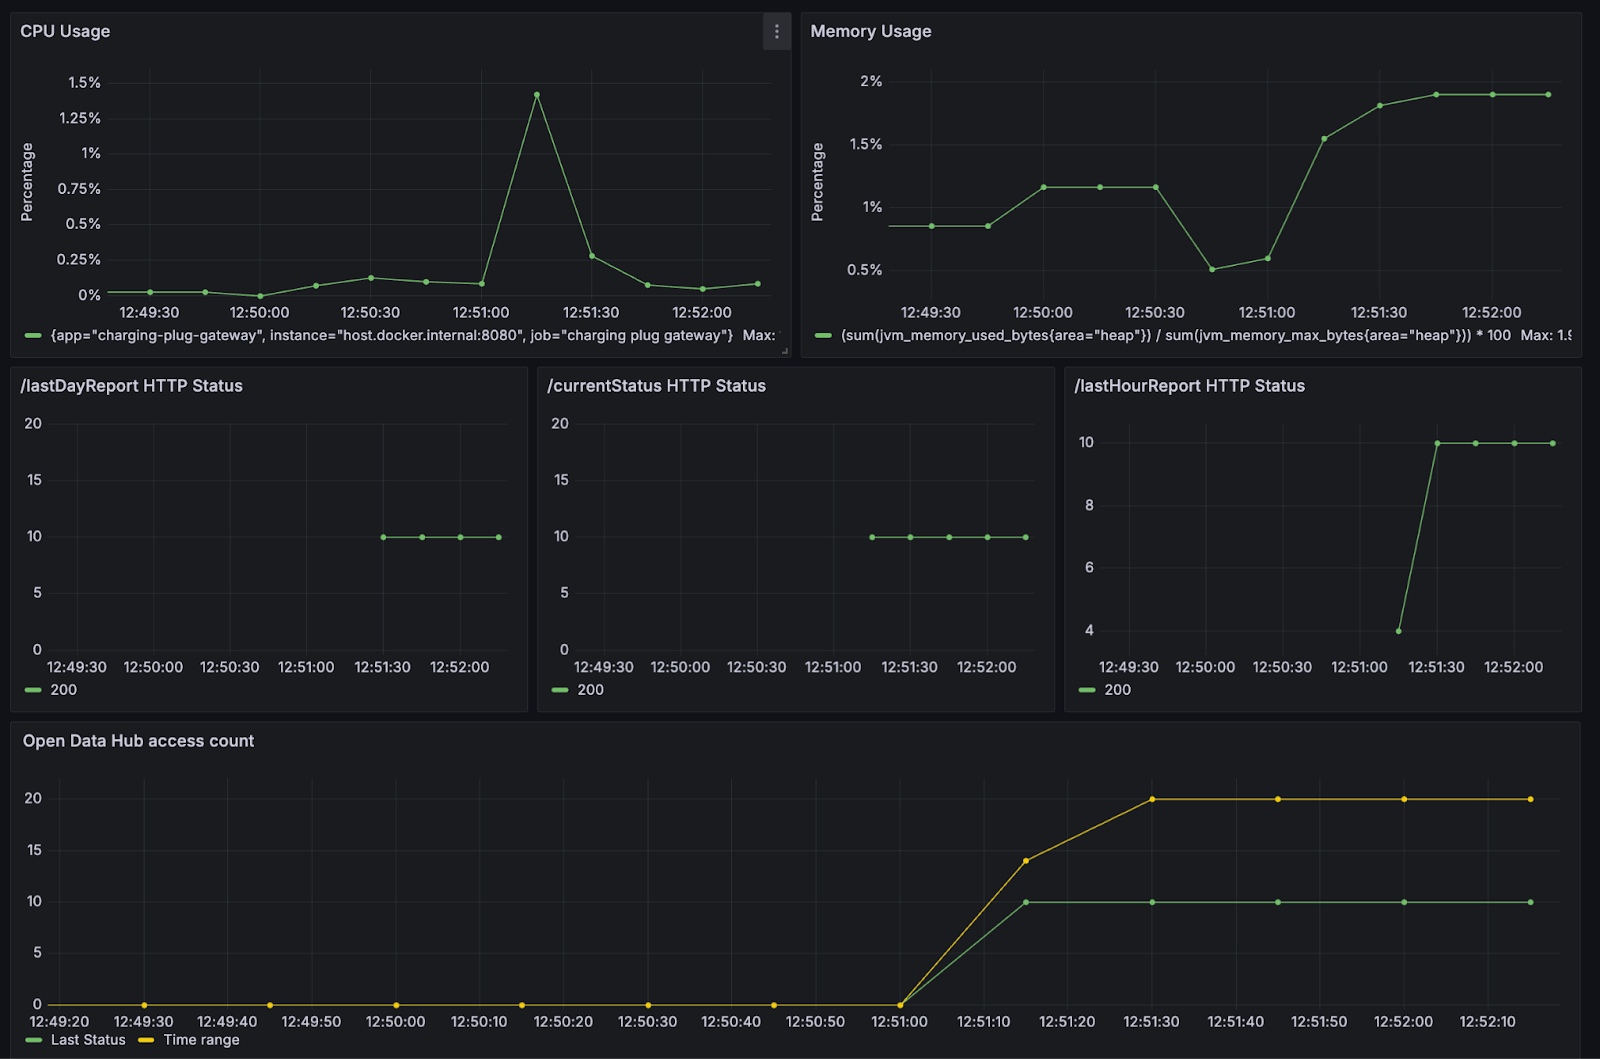
\includegraphics[width=1\textwidth]{polling10}
    \caption{Polling gateway experiment with 10 clients per feature runtime metrics.\label{fig:polling10}}
\end{figure}

In regards to figure~\ref{fig:polling10}: The first line contains charts of CPU and memory usage by the application during the experiment, notice that the CPU peaks on the moments the requests are received (12:51:00). On the second line, there are charts with the HTTP status of the response for each endpoint. In this case, the application was able to respond to all requests successfully, represented by the 200 OK status code. The third line contains a chart with the amount of data access made to the Open Data Hub, the data source, by the type of query. The current status feature uses the last status query, while last hour and last day report uses the time range query. For this reason, there is the double of time range queries made than the last status. 

\begin{figure}
    \centering
    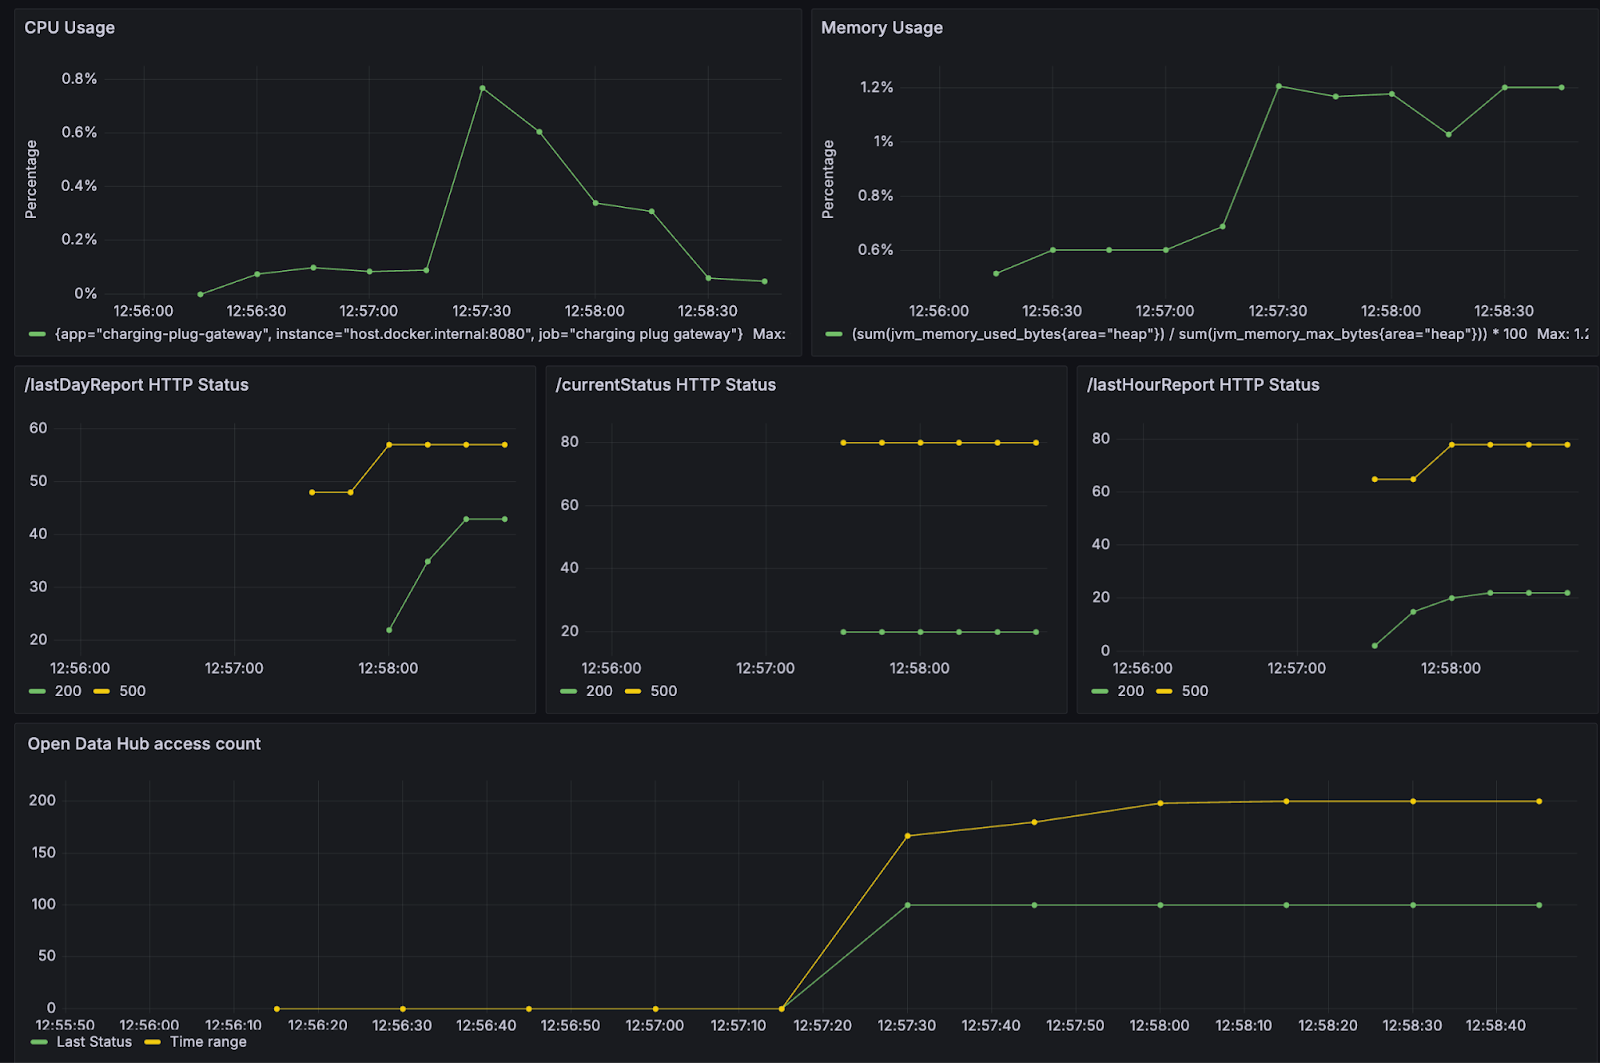
\includegraphics[width=1\textwidth]{polling100}
    \caption{Polling gateway experiment with 100 clients per feature runtime metrics.\label{fig:polling100}}
\end{figure}

In regards to figure~\ref{fig:polling100}: In this case, the data provider fails to respond around 70% of the clients, represented by the amount of 500 status code on the requests responses for each endpoint.

\begin{figure}
    \centering
    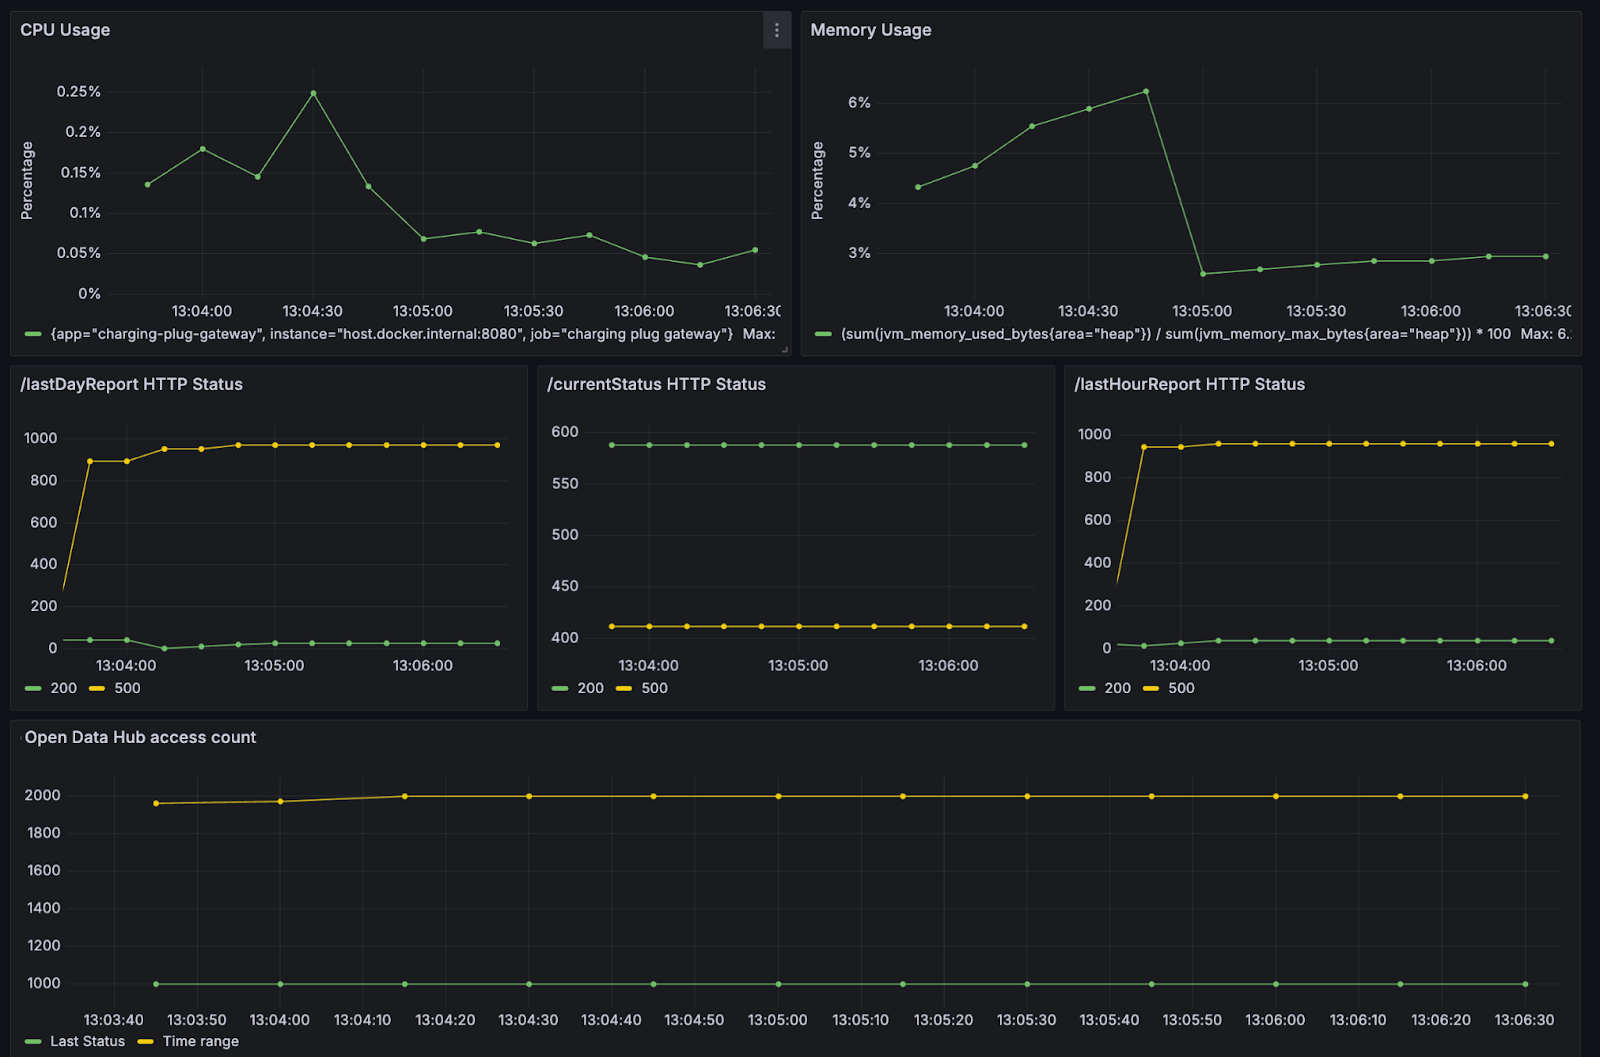
\includegraphics[width=1\textwidth]{polling1000}
    \caption{Polling gateway experiment with 1000 clients per feature runtime metrics.\label{fig:polling1000}}
\end{figure}

In regards to figure~\ref{fig:polling1000}: During this execution, the provider failed to respond to almost 80% of requests.

Notice that, in all executions, the CPU peaks during the requests handling. The memory usage tends to increase as the amount of requests increase and, consequently, the amount of objects to handle in memory. Also note that the amount of data lake access increases with the number of requests, since for each incoming request, the data gateway makes a new query on the data source.

\subsection*{Broadcaster gateway}
\label{sec:broadcasterresult}

The code necessary to implement the new feature at the Broadcaster gateway is at https://github.com/gfmota/charging-plug-gateway/pull/7 (Figure~\ref{fig:broadcasterdif})

\begin{figure}
    \centering
    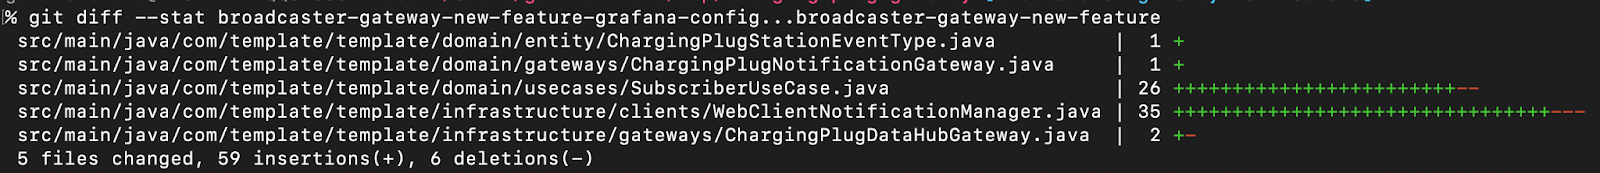
\includegraphics[width=1\textwidth]{broadcasterdif}
    \caption{Broadcaster gateway extension code diff.\label{fig:broadcasterdif}}
\end{figure}

The experiment consists of a client sending 10, 100 and 1000 requests per feature to the /subscribe endpoint at the gateway, subscribing itself to the gateway. Furthermore, on a CronJob trigger, it sends requests to every subscribed client with the requested data.

\begin{figure}
    \centering
    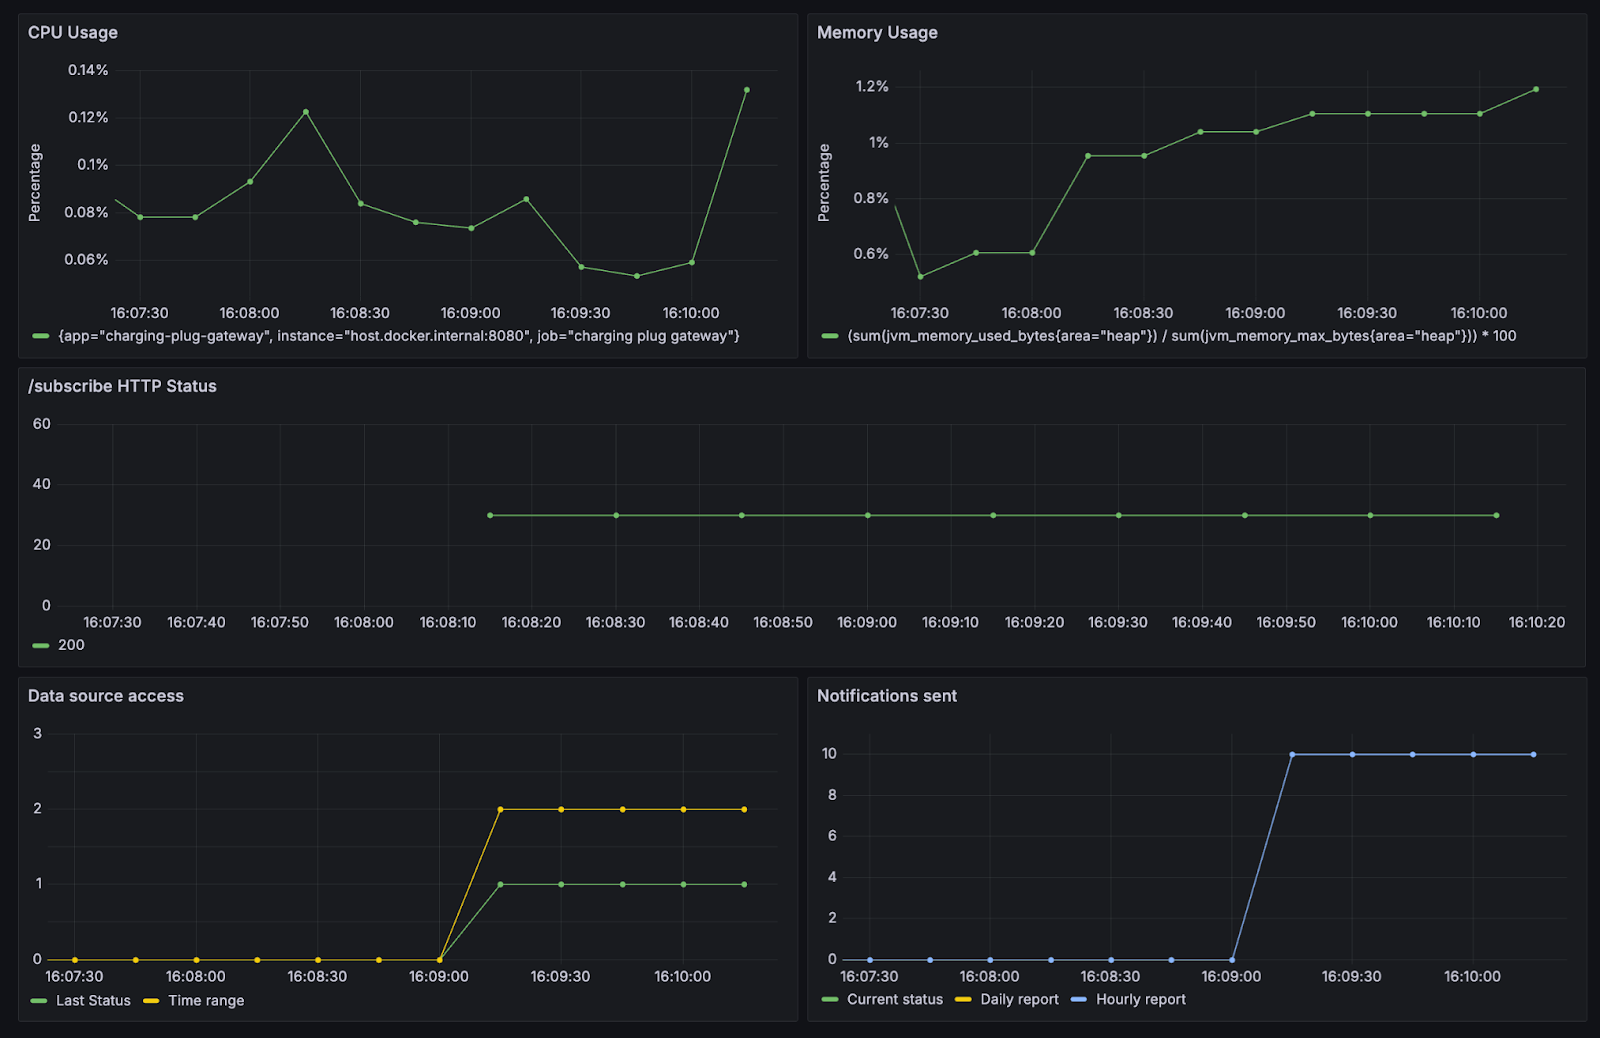
\includegraphics[width=1\textwidth]{broadcaster10}
    \caption{Broadcaster gateway experiment with 10 clients per feature runtime metrics.\label{fig:broadcaster10}}
\end{figure}

In regards to figure~\ref{fig:broadcaster10}: The first line is the same as in the previous scenario. The second line is a chart with the HTTP status of the response for the subscription endpoint. It shows there were 30 subscriptions, and on the next trigger, the notifications are sent for the services subscribed, as shown in the third line that contains charts for the data access made on Open DataHub and the amount of notifications sent for each type of data.

As the trigger was at the same moment for the three type of notifications, the lines on the notification sent chart overlapped, this means that the notifications were sent at the same moment and in the same amount.

In the last line the charts shows that no matter how many notifications are sent, it is required to retrieve data only once per type of notification, once in last status to notify the current status and two time range data access for hourly and daily notifications, as stated on the last scenario.

\begin{figure}
    \centering
    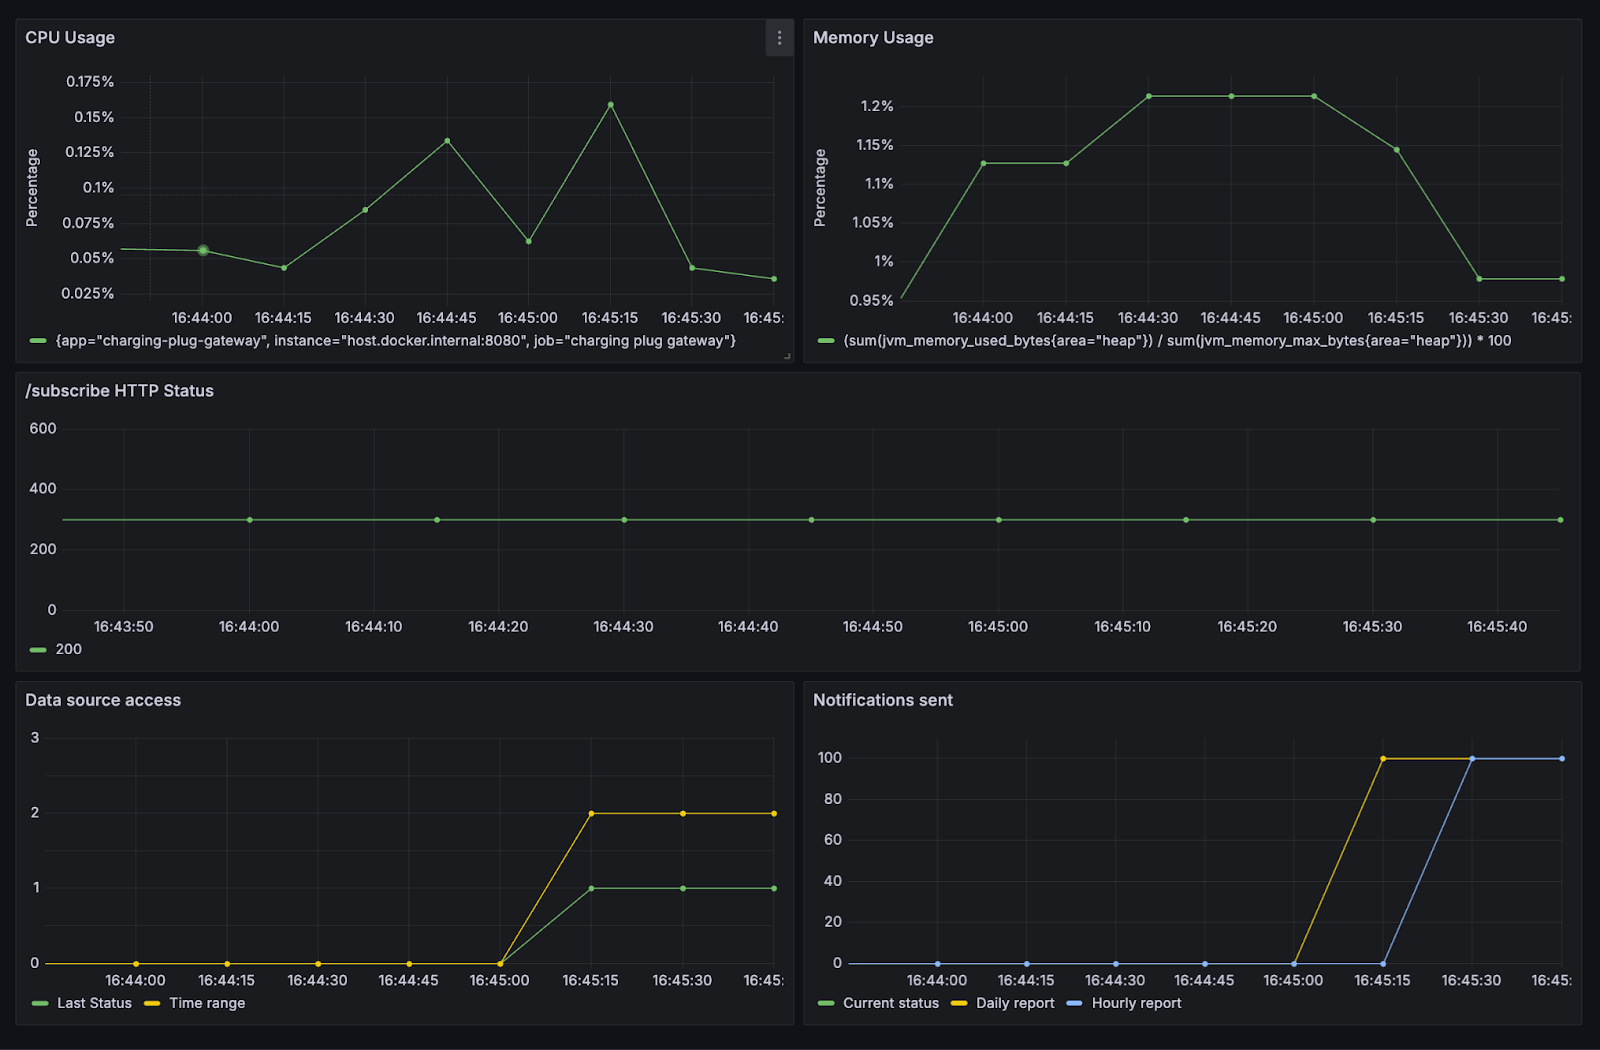
\includegraphics[width=1\textwidth]{broadcaster100}
    \caption{Broadcaster gateway experiment with 100 clients per feature runtime metrics.\label{fig:broadcaster100}}
\end{figure}

\begin{figure}
    \centering
    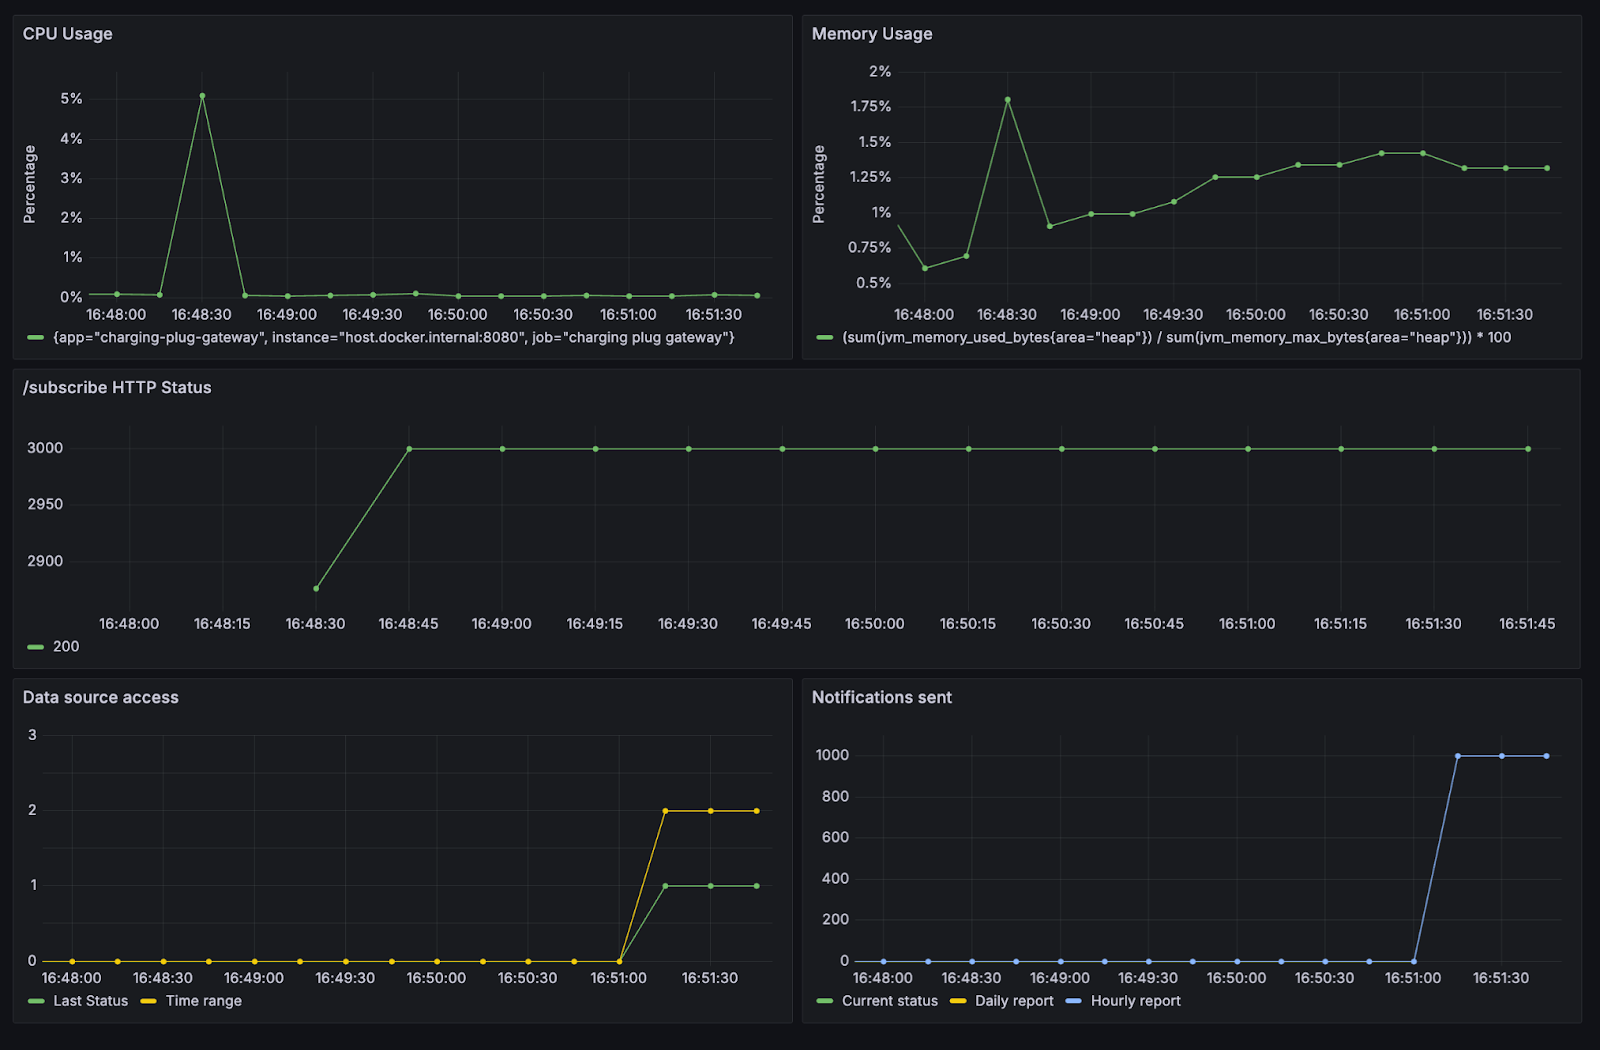
\includegraphics[width=1\textwidth]{broadcaster1000}
    \caption{Broadcaster gateway experiment with 1000 clients per feature runtime metrics.\label{fig:broadcaster1000}}
\end{figure}

In regards to figure~\ref{fig:broadcaster1000}: On this execution, it is possible to observe how the amount of notifications sent affect the application. The CPU and memory usage peaks as it receives a large amount of subscription requests, as happens in the first scenario with an HTTP handler. However, in this execution, the memory also peaks during notification, this happens because each notification requires an HTTP connection, each connection requires memory, this can be detrimental as the amount of notifications sent increases.

\subsection*{Message queue-based gateway}
\label{sec:messageresult}

The code necessary to implement the new feature at the Message queue-based gateway is at https://github.com/gfmota/charging-plug-gateway/pull/8 (Figure~\ref{fig:messagedif})

\begin{figure}
    \centering
    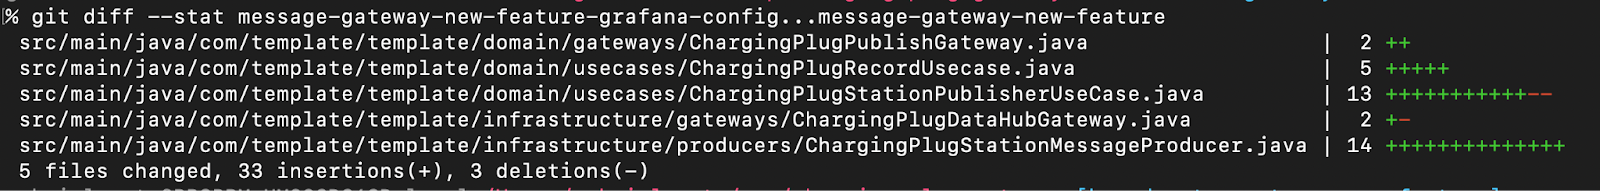
\includegraphics[width=1\textwidth]{messagedif}
    \caption{Message queue-based gateway extension code diff.\label{fig:messagedif}}
\end{figure}

The experiment consists of a client creating 10, 100 and 1000 queues per feature and attaching it to the topic created by the gateway. For each queue, the client creates a consumer to simulate multiple independent clients. On a CronJob trigger, the gateway sends a message per feature to the topic.

\begin{figure}
    \centering
    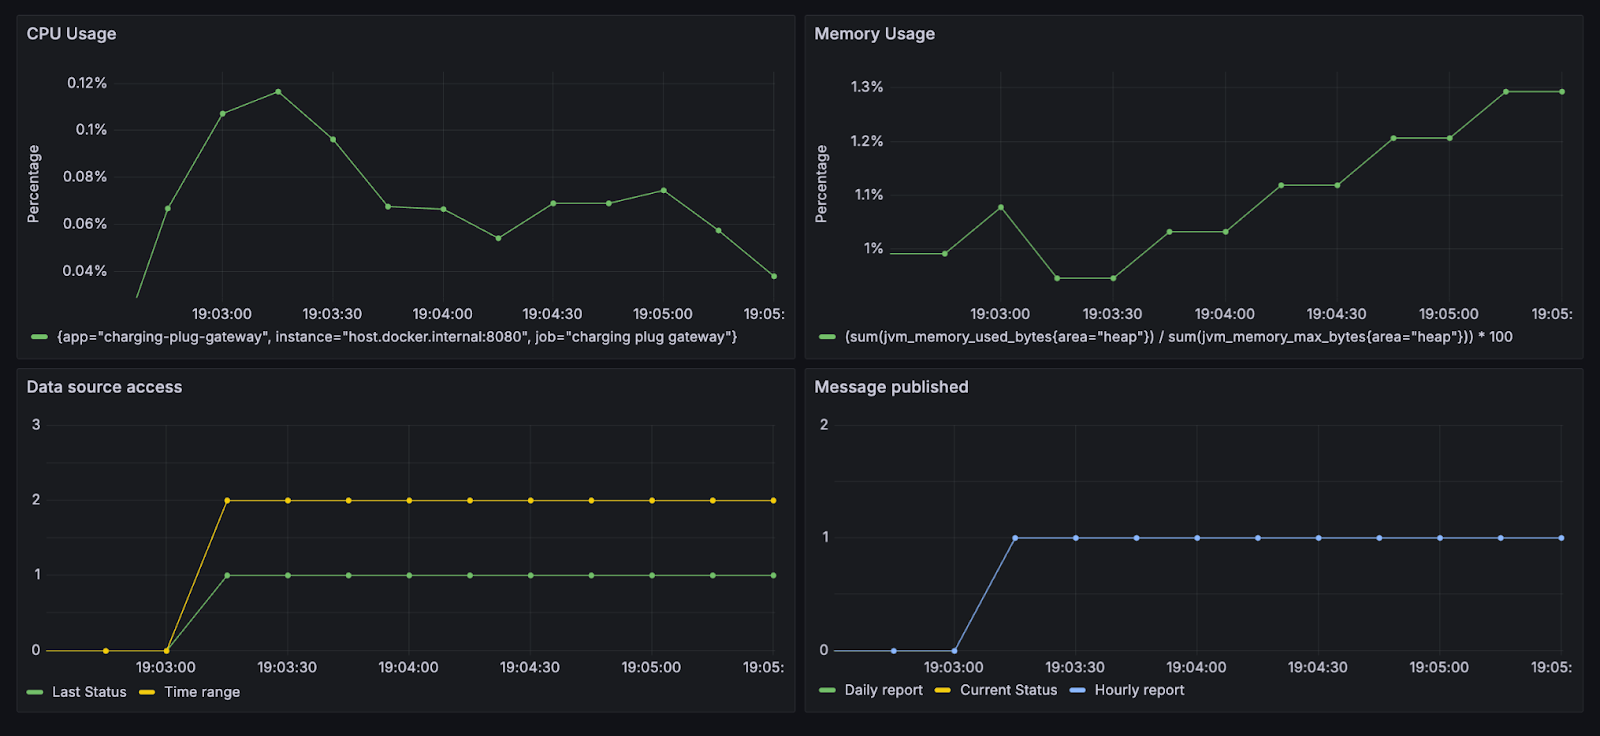
\includegraphics[width=1\textwidth]{message10}
    \caption{Message queue-based gateway experiment with 10 clients per feature runtime metrics.\label{fig:message10}}
\end{figure}

In regards to figure~\ref{fig:message10}: The first line contains are the same as described in the precious scenarios. In the second line, there is a chart of the amount of data access to source per type of data queried, remembering that daily and hourly features requires access to time range data and current status requires access to last status data. There is also a chart with the amount of messages published per type of message or feature. As happened in the previous scenario, the messages are sent at the same time, for this reason the lines in the chart may overlap.

\begin{figure}
    \centering
    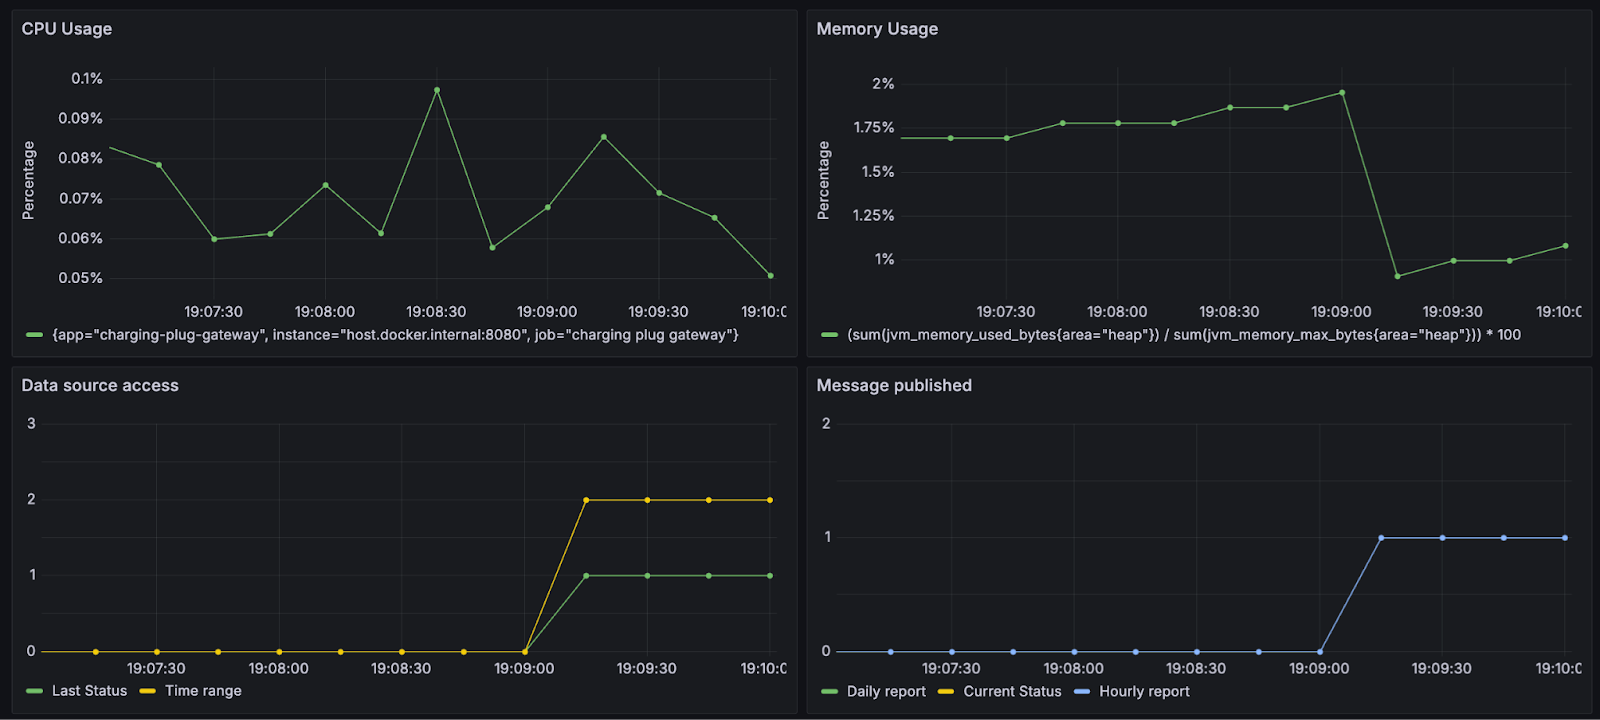
\includegraphics[width=1\textwidth]{message100}
    \caption{Message queue-based gateway experiment with 100 clients per feature runtime metrics.\label{fig:message100}}
\end{figure}

\begin{figure}
    \centering
    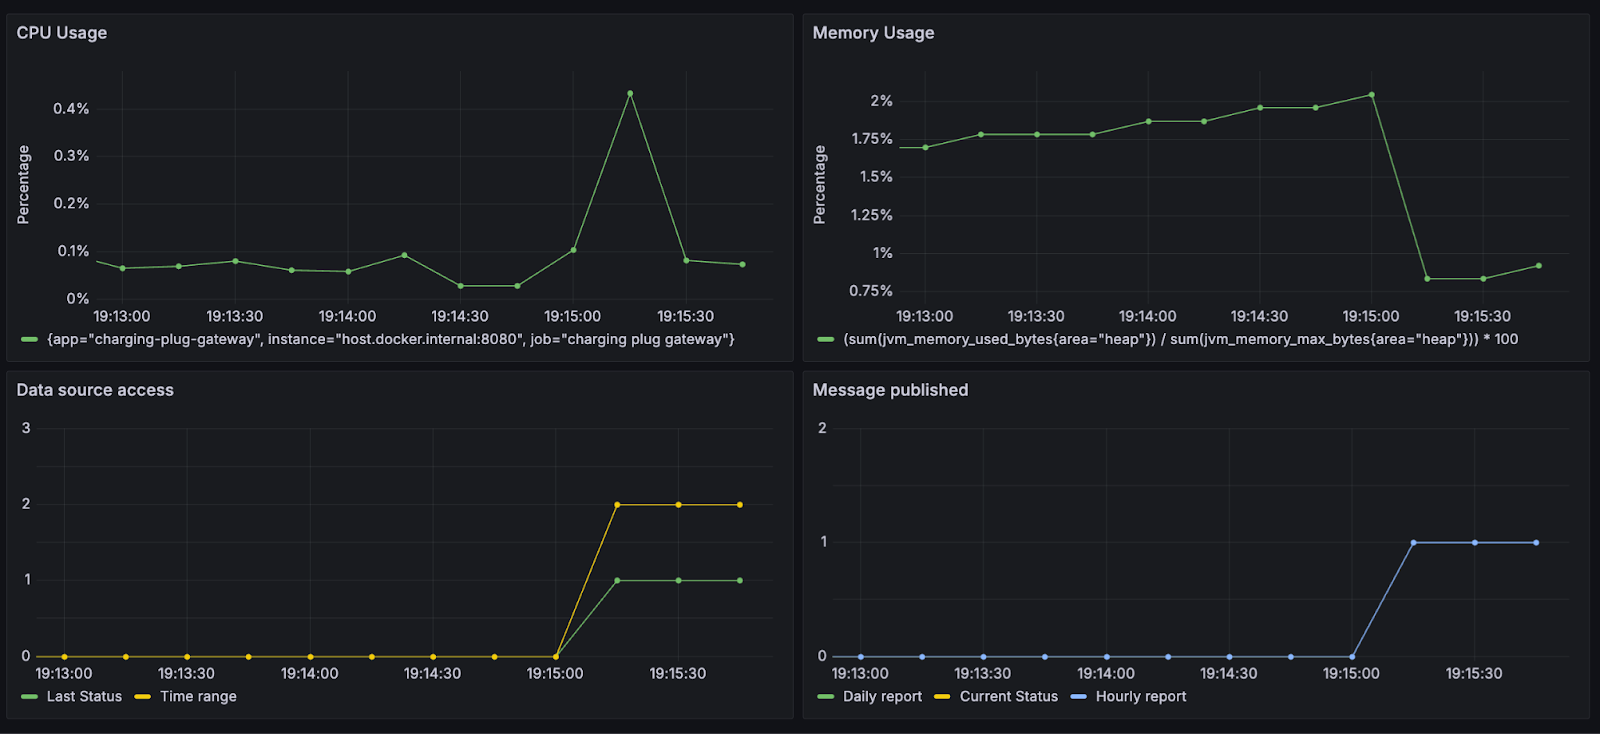
\includegraphics[width=1\textwidth]{message1000}
    \caption{Message queue-based gateway experiment with 1000 clients per feature runtime metrics.\label{fig:message1000}}
\end{figure}

Notice that, as in the Broadcaster, there is only one data source access per feature per trigger, however, for each trigger, only one message is sent per feature, no matter how many data consumers are served. This also means that the CPU and memory usage is close to equal for all executions.

\section{Takeaways}
\label{sec:providerconclusion}

After the experiments, it's possible to take some conclusions about each scenario according to extensibility.

\subsection*{Extensibility and Development experience}
\label{sec:devex}

When looking for number of code changes at the git diff for each scenario, the Polling Gateway had the least line changes for the base implementation and for feature addition.

However, all have similar work necessary to add new features, and the base implementation depends on how comfortable the developer is with the infrastructure used. On the perspective of a junior developer, synchronous communication with HTTP can be easier, since it is more common and thus used a base concept for multiple subjects, such as web development. While message broker and asynchronous communication are advanced concepts and require more complex tools and knowledge, what can end up intimidating these developers.

\subsection*{Data source usage}
\label{sec:source}

The chart of data source accesses shows that the Broadcaster and Message queue-based gateway use a constant number of data access independent of the number of clients. Meanwhile, the Polling gateway has to access the data source every time it receives a request, even thought the result hasn’t changed.

This characteristic of the polling gateway can be detrimental to the application environment since each request depends on I/O, adding response time, and leading to unnecessary computation by the data source service.

To minimize these, it is possible to use cache on data source calls. On the experiment use case, it was necessary to implement an in-memory cache, due to the data source being a third-party open API. 

However, the in-memory cache is not recommended in all cases, for example in big applications, where it is likely to have multiple Pods running the same application, each Pod has its own memory and can't share it with others. Therefore, in-memory cache wouldn't be 100% effective and can be replaced by a more robust solution. There are different types of caches and the choice depends on the effective needed and the budget available for infrastructure solutions.

Using cache would also imply on the infrastructure cost increase. The cost can vary depending on the tool, it can be cheap as in-memory cache, or higher using a fast access database.

\subsection*{Scalability}
\label{sec:scala}

Scalability is used in regard to how well each scenario deals with the increase of clients. At first, the Polling gateway seems the least scalable, with the client number increase, it started to have fail to deal with the requests and throwing error to clients. It means that clients of the Polling gateway needs to have some fallback mechanisms, like retry implementation.

It is possible to minimize it by adding horizontal scaling and load balancing, doing so would be able to distribute requests and thus processing required. However, this would require an increase in cost and in infrastructure complexity.

Due to the nature of the Broadcaster gateway to only send requests from time to time, with a cron job or observing updates on the data source, it has low CPU usage for most of the time. However, when it starts the process to notify the subscribed clients, the CPU usages increase according to the number of clients, since each one needs a request.

There are also considerations about the subscription method. The subscribe endpoint can end up having  problems with availability if it receives a big volume of requests at the same time, as in the Polling gateway. Even thought, this endpoint is not planned to have high usage, there should be worry about how to deal with lost requests.

It is also important to have safe unsubscribe methods. It can help avoid sending unnecessary requests and thus saving CPU usage.

While the Message queue-based gateway have the same behavior of the Broadcaster according to when it sends data to clients, it doesn't peak CPU usage during processing data and publishing messages, thus can be said the best solution to scale. This is because the gateway have constant processing no matter how many clients it is serving, since it can serve multiple clients with a single message.

\subsection*{Client autonomy}
\label{sec:client}

Another point to take in consideration when comparing each scenario, is how much each client is attached to the gateway solution. The Broadcaster experiment have an example of an attached client.

The Broadcaster's client needs to have an HTTP endpoint available all the time for gateway updates. For this reason, it is important to the Broadcaster gateway to add a failure mechanism, such as retry implementation, in case the client is unavailable or with high traffic.

\begin{figure}
    \centering
    \includegraphics[width=.8\textwidth]{Gateway-Página-3.drawio}
    \caption{Broadcaster gateway dependency diagram.\label{fig:subfigures6}}
\end{figure}

The Polling gateway shows what a bad autonomy is. The client is autonomous to request the data it wants whenever it needs. It can save CPU usage sometimes, since, if there is no request, there is no need for the gateway to retrieve data and process it. However, as it is the client's responsibility to request the data, there is no way for the client to know if there is a data update. This can cause the client to request multiple times for the same data, wasting both gateway and client processing capability with repeated data.

\begin{figure}
    \centering
    \includegraphics[width=.8\textwidth]{Gateway-Página-2.drawio}
    \caption{Polling gateway dependency diagram.\label{fig:subfigures7}}
\end{figure}

While the Message queue-based gateway have the best example of autonomy. The client service does not need to be available for the gateway, since the queue can store the messages until they are consumed. The client can also consume the data from the queue whenever it wants, but only if it is an update available, otherwise there will be no message on the queue, avoiding consuming repeated data as in the Polling scenario.

\begin{figure}
    \centering
    \includegraphics[width=.8\textwidth]{Gateway-Página-4.drawio}
    \caption{Message queue-based gateway dependency diagram.\label{fig:subfigures8}}
\end{figure}

\subsection*{Infrastructure cost}
\label{sec:infra}

Each scenario have its own environment and needs. As in a software system, it is important to consider the cost in regard to all services used by an application, each service requires maintenance and have a cost attached to it.

In this regard, the Polling gateway may seen ahead because in the first implementation there is no need of extra services to support it. However, as discussed previously, this is not true when scalability is necessary, requiring cache tools and horizontal scaling to perform well on high usage scenarios.

The Broadcaster gateway requires only a database to store the clients subscribed to the service. For this reason, it is important to create routines to keep the data clean of unused information and a good indexing to minimize IO time. It is important to note, as mentioned previously, for each notification sent it is necessary to create a new HTTP connection, connections use network bandwidth, this can become a problem as the amount of clients increase and cause increasing cloud cost as the bandwidth used get larger.

The Message queue-based requires a message broker for the implementation, but also is the only one that requires a message broker on the client side. This can be trick when dealing with multisource clients, depending on the use case.

\newcommand{\sla}{\textbackslash}

\newcommand{\cmd}[1]{\textsf{#1}}

\newcommand{\pkg}[1]{\textsf{#1}}

\newcommand{\ltxcmd}[1]{\cmd{\sla{}#1}}

\chapter{Data Ingestion Study Case}
\label{chap:dataingestion}

\section{Introduction}
\label{sec:introductioning}
OpenDataHub (ODH) is a digital platform that makes data from different sources available in a standardized pattern, removing the complexity of integrating multiple data sources for the users\footnote{Reference from OpenDataHub's webpage https://opendatahub.com/}. The full picture of their system can be split into three functionalities:

\begin{itemize}
    \item Data ingestion: applications responsible for retrieving or receiving data from external data sources, identifying, transforming, and storing it.
    \item Data storage: the data is stored in a stations-values format  – stations are complex objects that have a type and can contain other stations or properties, a list of numeric values followed by data that describe it, such as value name and measurement unit\footnote{Reference OpenDataHub's documentation https://opendatahub.readthedocs.io/en/latest/howto/mobility/getstarted.html#getting-started}. For example, a charging plug station is a station that contains plugs, each plug is a station that contains a value ”available” or “not available”. Stations can contain more than one value, for example, a latitude-longitude point is a station that contains values for wind speed, wind direction, air pressure, and others. These values are stored in the same unit for every station, no matter the original data source unit and format.
    \item Data exposure: a common API to make data from stations available for end users.
\end{itemize}

This case study focuses on the data ingestion architecture, and how to increase its extensibility.

\begin{figure}
    \centering
    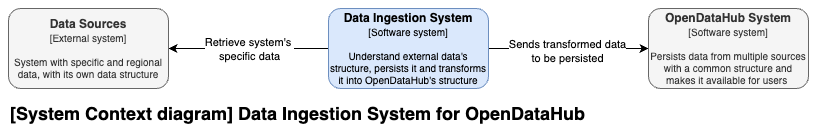
\includegraphics[width=1\textwidth]{collector-consumer-CONTEXT.drawio}
    \caption{Data Ingestion context diagram.\label{fig:subfigures9}}
\end{figure}

\section{Current architecture}
\label{sec:current}

The ODH's data collectors architecture's initial requirement is to connect to different data sources, using different protocols (e.g. HTTP APIs, MQTT, FTP) to download the data, aggregate and transform it to the stations-value pattern, and save it on ODH’s storage.

The current architecture uses independent applications dedicated to each data source. Each application is responsible for connecting to the data source, retrieving the data, aggregating and/or transforming it, and sending it to ODH's system for persisting data.

\begin{figure}
    \centering
    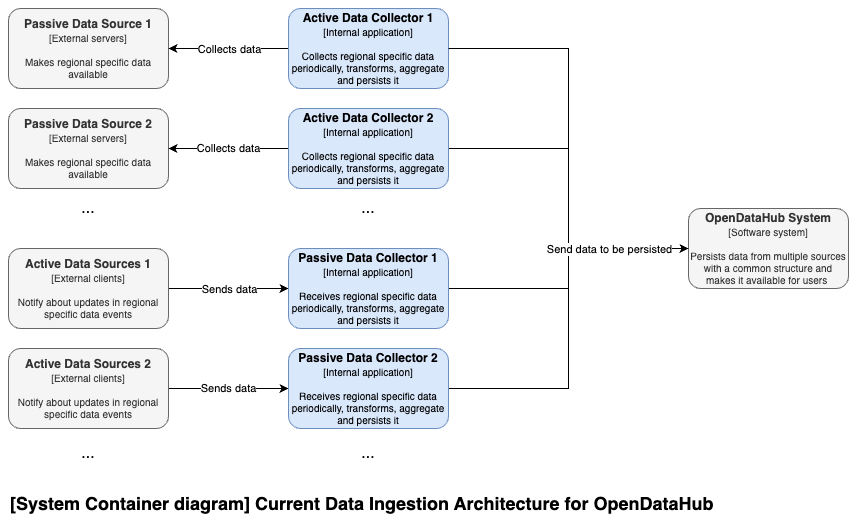
\includegraphics[width=1\textwidth]{collector-consumer-OLD CONTAINERS.drawio}
    \caption{Data Ingestion current architecture containers diagram.\label{fig:subfigures10}}
\end{figure}

This solution contains a problem of redundant work for each data collector service: they all have code to connect with the ODH's persistence system and might benefit from reusing processing and transformation tooling. This creates N dependencies with the storage, consequently, if there is a change in how the connection with the ODH's persistence system is made, it would require changing every data collector.

Besides, to integrate a new data source into the data collection, it is necessary to create a new service for collecting, parsing, transforming, and persisting code.

\section{New requirements}
\label{sec:requirements}

As a growing platform, ODH wants to be able to integrate new data sources with ease, decreasing technical requirements and development time. As part of this, it is essential to provide a way for data sources' teams to integrate with ODH's data collection, without requiring (or at least reducing) ODH's technical team involvement.

Furthermore, it is essential to have a way to track and debug the ingestion flow. For this reason, another requirement is to integrate a new database to store the “raw” data, which means, the data as it is collected before it is transformed into the ODH stations pattern.

For this, the current architecture would require each data collector application to connect to the raw data storage and store it. Creating another dependency coupling problem, since every data collector would require a dependency with the Raw data storage.

\section{Proposed architecture}
\label{sec:proposed}

The new architecture proposed in this thesis aims to increase the system's extensibility by reducing development time to create new data collectors. With it, it creates an option for data sources that want to integrate in, reducing ODH's technical team involvement and removing data collectors coupling with storage systems.

The new architecture uses microservices and asynchronous communication to modularize and split concerns along the system. (Figure~\ref{fig:containers})

\begin{figure}
    \centering
    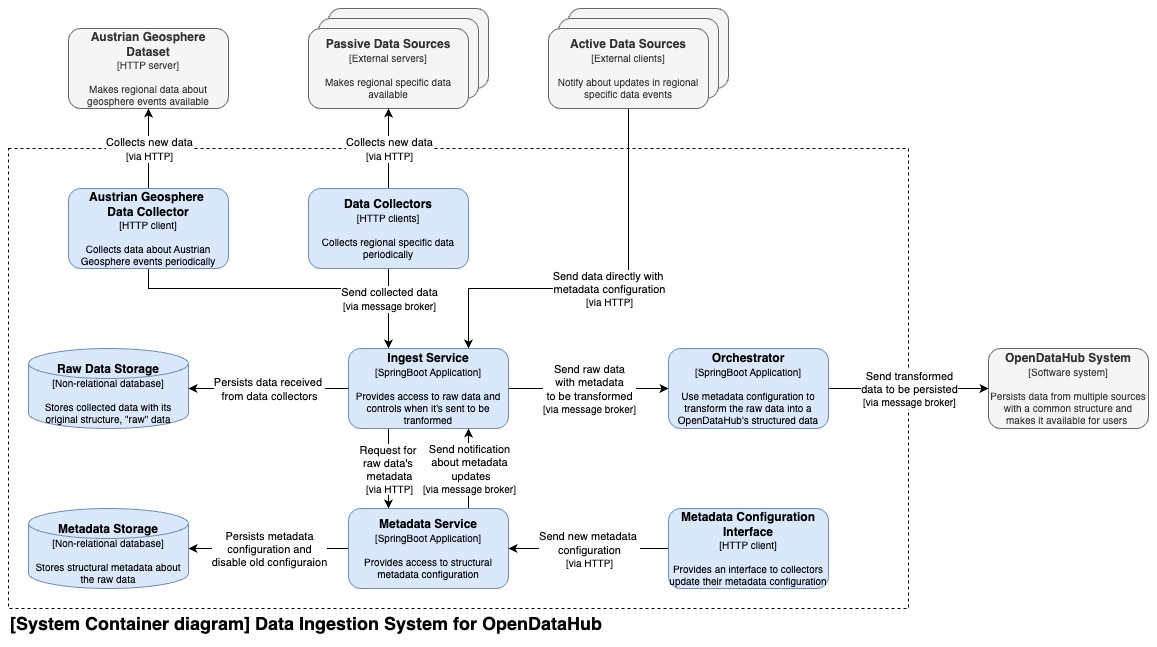
\includegraphics[width=1\textwidth]{collector-consumer-CONTAINERS.drawio}
    \caption{Data Ingestion proposed architecture containers diagram.\label{fig:containers}}
\end{figure}

The biggest challenge in this architecture is: How to treat external data and their singularities. Each data source has its data format and structure, how to extract the information needed by ODH and transform it into the expected pattern?

It can be solved with structural metadata, metadata is a kind of data used to describe data, in this case, it will contain information about the data structure: in which field is an important value, what are the data types, and how to access each wanted value.

This metadata can be sent with the data or configured, in case the same metadata can be used multiple times and is needed for the transformation process.

\subsection{Ingestion}
\label{sec:ingestion}

The data ingestion is done by the Ingestion Service. It is responsible for receiving the raw data from data collectors or active data sources (data sources sending the data directly to it), persisting this data into a raw data storage, and sending data to be transformed.

Data can only be sent to be processed once there is a metadata configuration to it. This metadata can be sent with the data, or be fetched from the Metadata Service (application responsible for handling metadata operations).

However, the raw data persistence does not depend on the metadata configuration. This means that data received without metadata or any metadata configuration will be persisted on Raw Data Storage and sent for transformation once the metadata is configured. For this reason, there is a dedicated worker to listen for metadata update messages and trigger this process. (Figure~\ref{fig:ingest})

\begin{figure}
    \centering
    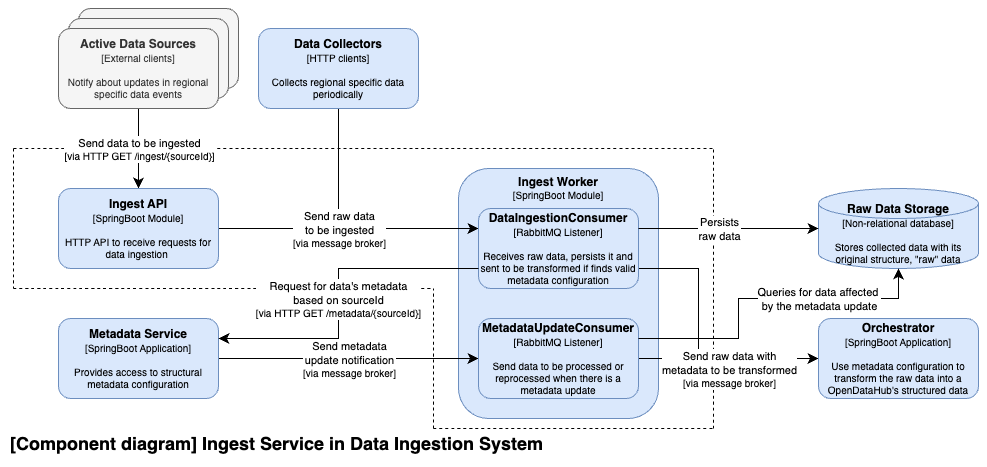
\includegraphics[width=1\textwidth]{collector-consumer-COMPONENT INGEST.drawio}
    \caption{Ingestion service components diagram.\label{fig:ingest}}
\end{figure}

\subsection{Metadata}
\label{sec:metadata}

The solution uses structural metadata about the data ingested to transform data from its raw structure into the ODH's station pattern. This metadata can be sent or collected with the data or can be configured to be applied to data collected during a time range(~\cite{Metadata}).

There is a metadata storage to store active configurations and to help debugging. The application dedicated to handling access and operations on the storage is the Metadata Service.

There is also a Metadata Configuration Interface to help developers and data sources configure new metadata and manage their data configuration. (Figure~\ref{fig:metadata})

\begin{figure}
    \centering
    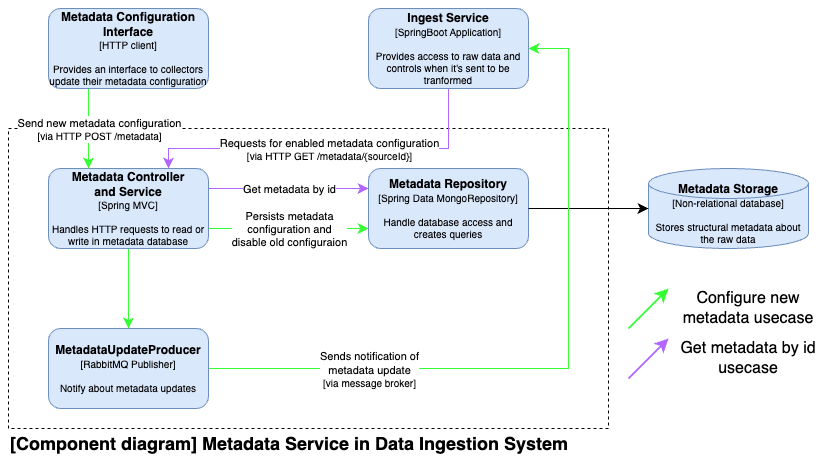
\includegraphics[width=1\textwidth]{collector-consumer-COMPONENT METADATA.drawio}
    \caption{Metadata service components diagram.\label{fig:metadata}}
\end{figure}

The metadata is built with a common structure and stored as a JSON. Follows an example of metadata in Program~\ref{prog:metadata}.

\begin{program}
    \index{JSON}
    \centering
  
  \begin{lstlisting}[language=JSON, style=wider]
{
 "sourceId": "austrian-geosphere",
 "startDate": "2015-08-04T10:11:30",
 "expirationDate": "2029-08-04T10:11:30",
 "metadata": {
 "dataId": "austrian-geosphere-data",
 "origin": "austrian-geosphere-data-collector",
 "period": 600,
 "timestampProperty": "timestamps.0",
 "results": {
 "type": "array",
 "property": "features",
 "idProperty": "properties.station"
 },
 "stations": {
 "type": "array",
 "property": "features",
 "identification": {
 "property": "properties.station"
 },
 "location": {
 "property": "geometry.coordinates",
 "type": "array",
 "longitude": "0",
 "latitude": "1"
 }
 },
 "datatypes": [
 {
 "datatypeName": "air_pressure",
 "method": "extract",
 "unitProperty": "properties.parameters.P.unit",
 "valueProperty": "properties.parameters.P.data",
 "targetUnit": "hPa",
 "rtype": "mean"
 },
 {
 "datatypeName": "wind_speed",
 "method": "extract",
 "unitProperty": "properties.parameters.FF.unit",
 "valueProperty": "properties.parameters.FF.data",
 "targetUnit": "m/s",
 "rtype": "mean"
 },
 {
 "datatypeName": "wind_direction",
 "method": "extract",
 "unitProperty": "properties.parameters.DD.unit",
 "valueProperty": "properties.parameters.DD.data",
 "targetUnit": "°",
 "rtype": "mean"
 },
 {
 "datatypeName": "wind_temperature",
 "method": "extract",
 "unitProperty": "properties.parameters.TL.unit",
 "valueProperty": "properties.parameters.TL.data",
 "targetUnit": "°F",
 "rtype": "mean"
 }
 ]
 }
}
  \end{lstlisting}
  
    \caption{Structural metadata for Austrian Geosphere dataset.\label{prog:metadata}}
\end{program}

The content describes how the data structure and in which keys are key values for the data transformation, for example: the timestamp of the event, the event location, and the value registered.

\subsection{Transformation}
\label{sec:transformation}

The data transformation is done by the Orchestrator, once it receives data with its metadata configuration. The Orchestrator uses the metadata to understand the particularities of the raw data and transform it into the ODH's station structure.

The Orchestrator is not only responsible for transforming the data structure to match the expected structure but also for transforming the collected value into the expected unit of measurement. Since the data is stored in the same unit to ease end users. It can do so, by using the Transformers.

Transformers are small pieces of code that do only one transformation into the value. For example, there may be a Transformer to transform a temperature value measured in Celsius to Kelvin. The Orchestrator is responsible for selecting the correct Transformers and running them into the correct order to transform from the collected unit to the one used by ODH's system. (Figure~\ref{fig:orchestrator})

\begin{figure}
    \centering
    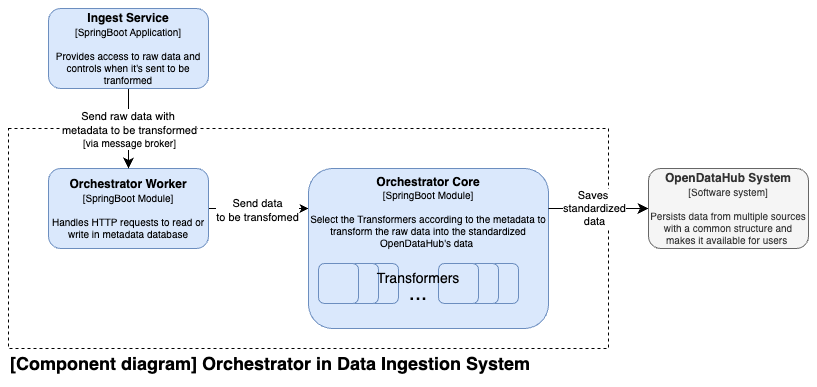
\includegraphics[width=1\textwidth]{collector-consumer-COMPONENT ORCHESTRATOR.drawio}
    \caption{Orchestrator components diagram.\label{fig:orchestrator}}
\end{figure}

\section{Experiment}
\label{sec:exp}

There is an experiment to test the proposed architecture. It simulates the integration of an Austrian geosphere data source, it ingests data on current air pressure, temperature, wind speed, and direction in different points from Austria. The data is collected every 10 minutes, the time the data source takes to update its values. This experiment aims to only simulate the data ingestion process and not send data to be persisted in the ODH system, but it allows observing the products of data ingestion and how each microservice relates and communicates with each other.

The experiment is in a GitHub repository as a Gradle monorepo, each service is a submodule of the repository, but each one can be deployed individually as a microservice, they are in Java 17. They use SpringBoot to create HTTP APIs and asynchronous workers. For infrastructure, it uses MongoDB for data storage and RabbitMQ for asynchronous communication via message queues.

To run the experiment, it is necessary to first prepare the environment, then run the infrastructure; after that, run the microservices, and finally include test metadata. It is also possible to simulate an active data source and send data directly to it to be ingested. This process is described step-by-step on the repository's README.

To access the HTTP endpoints, it is possible to use the Postman collection available in the repository, to act as an interface for debugging, active data ingestion, and/or metadata configuration.

During the experiment run, the applications logs are directed to files in the log folder to ease debugging and tracking. It is also possible to access the MongoDB, to track the data stored, and the RabbitMQ, to track messages and queues, servers by using the values in the docker-compose file.

\section{Takeaways}
\label{sec:conc}

It is possible to evaluate the extensibility of a data ingestion system by how easy it is to integrate different data sources and give maintenance to it.

On the current architecture, integrating a different data source would require creating a new application that would collect the data, transform and send it to ODH. Every time the data changes, it would require a change in the code base, this requires effort from the ODH's technical team and alignment between ODH and the data source owners.

The proposed architecture uses microservices and the concept of modularity to split the responsibility between the systems in different microservices. Also uses structural metadata to abstract transformation logic from the data collector.

For these reasons, integrating a new data source on the proposed architecture requires less technical work, once it is possible to be integrated by the own data source, via the ingestion API, or requires a data collector service that only contains code related to data collecting.

Also, maintaining the data sources is much easier, since data changes can be instantly met in the transformation process by changing the metadata configuration, which can be done by the data source team, via the metadata service API, reducing ODH technical team involvement.

Another advantage brought by the proposed architecture is the use of asynchronous communication. This reduces coupling problems, once the message publisher doesn't have any dependency with the consumer application. It also increases scalability, by reducing the harm of overload scenarios, since the messages are stored and only processed by the consumer once it is available.

A further improvement of the proposed architecture is the split of ingestion and transformation flows. Ingestion is the process of collecting the data and persisting it in the Raw Data Storage, and transformation is the process of using metadata to transform raw data into ODH's standardized data. Separating them means that data can be ingested even though they are not ready to be transformed (doesn't have a metadata configuration). This increases the data collecting capability, since it is not attached to the transformation logic, and reduces risks of data loss, once the data is stored and is going to be processed once the metadata is configured.

This also prevents unexpected behaviors on transformation from causing data loss, because the raw data is stored, and once the cause is found and fixed, the transformation can be triggered again.

Although there are many advantages to the proposed architecture, the use of asynchronous communication, microservices, and the addition of two data storage cause an increase in infrastructure cost and maintainability. For this reason, it is important to be sure there is an experienced team with microservices and the use of observability and tracking tools, such as Grafana, Prometheus, and Sentry, to make sure that the applications are healthy and working as intended and any unwanted behavior is caught and fixed as soon as possible.

\newcommand{\sla}{\textbackslash}

\newcommand{\cmd}[1]{\textsf{#1}}

\newcommand{\pkg}[1]{\textsf{#1}}

\newcommand{\ltxcmd}[1]{\cmd{\sla{}#1}}

\chapter{Conclusion}
\label{chap:conclusion}

This work studied two MSA case studies and explored different scenarios to find architectural characteristics that grant extensibility to the system. The first case study focused on a Data Provider that provides access to a data source for multiple clients, it was implemented in three different scenarios, that differ in communication methods, infrastructure components, and client responsibilities. In the second scenario, we focused on a Data Ingestion system, based on OpenDataHub's use case, that provides a port of entrance for data from multiple sources, with different structures and units, to be integrated into a single data storage system. It was made one architecture proposal, with implementation, and compared with their current approach.

The first case study provided a comparison of different approaches to client-server communication, synchronous and asynchronous communication methods, HTTP requests, and message broker queues. This made it possible to conclude that asynchronous communication via message broker allows for a higher level of extensibility and scalability because it doesn't create a direct dependency between the client and the provider. However, the use of asynchronous communication restricts the client's autonomy to fetch the data as needed, and this can be a downside for scenarios where clients have low data source usage.

The second case study provided an example of concern split, modularization, and generalization to increase extensibility. Splitting the system into small applications with a single responsibility allows for code reusability to increase and reduce work to add new features. Generalizing the transformation logic, by using structural metadata configuration, increases code reusability and reduces code changes needed to update features behavior.

Overall, both case studies exemplify how the use of asynchronous communication between services can help architectures increase extensibility and service autonomy. Because it makes it possible for services to communicate without worrying about which and when an application is going to handle the communication message.

Another concept utilized in both case studies is the use of data storage to perform tracking and reduce communication overhead by storing reutilizable data. Reducing the communication needed to perform an action for a new feature is key to increasing extensibility, once it reduces dependencies between services and code needed to add new features or update them.

In conclusion, this work exemplifies how the use of asynchronous communication between service and data storage for reusable data can increase the extensibility of a Microservice system's architecture. It also provides implementation examples, developer experience reports, and conclusions based on metrics collected in runtime.


%%%%%%%%%%%%%%% SEÇÕES FINAIS (BIBLIOGRAFIA E ÍNDICE REMISSIVO) %%%%%%%%%%%%%%%%

% O comando backmatter desabilita a numeração de capítulos.
\backmatter

\pagestyle{backmatter}

% Espaço adicional no sumário antes das referências / índice remissivo
\addtocontents{toc}{\vspace{2\baselineskip plus .5\baselineskip minus .5\baselineskip}}

% A bibliografia é obrigatória

\printbibliography[
  title=\refname\label{sec:bib}, % "Referências", recomendado pela ABNT
  %title=\bibname\label{sec:bib}, % "Bibliografia"
  heading=bibintoc, % Inclui a bibliografia no sumário
]

\printindex % imprime o índice remissivo no documento (opcional)

\end{document}
